\documentclass[fleqn]{beamer}

\usepackage[british]{babel}
\usepackage{graphicx,ru,url}
\graphicspath{{../tex/figures/}}
\usepackage{amsmath}
% Use Times for math font and text font.
\RequirePackage[T1]{fontenc}
%\RequirePackage{txfonts}
% bold math must be loaded after Times font
\usepackage{bm}
\usepackage{booktabs} % nice rules (thick lines) for tables
\usepackage{microtype} % improves typography for PDF
\usepackage{xcolor} % Allows colors in fonts

\usepackage{tikz} % Allows creation of tikz pictures
\usetikzlibrary{arrows}
\usetikzlibrary{arrows.meta}

\usepackage{verbatim}
\usetikzlibrary{arrows,shapes,snakes}
\usetikzlibrary{patterns}
\usepackage{url}
\usepackage{ifthen}
\usepackage{subcaption}
\usepackage{slashbox} % backslashbox in a table

% typesetting using the algorithmicx package
% detail at: https://en.wikibooks.org/wiki/LaTeX/Algorithms and https://tex.stackexchange.com/questions/229355/algorithm-algorithmic-algorithmicx-algorithm2e-algpseudocode-confused
\usepackage{algorithm}
\usepackage{algpseudocode}

\usepackage{multibib}
\newcites{Mypub}{List of Publications}

% The title of the presentation:
%  - first a short version which is visible at the bottom of each slide;
%  - second the full title shown on the title slide;
\title[KSU Beam Characterization]{Neutron Flux Characterization of the Kansas State University TRIGA Mark II's Northeast Beam Port}

% Optional: a subtitle to be displayed on the title slide
%\subtitle{Show where you're from}

% The author(s) of the presentation:
%  - again first a short version to be displayed at the bottom;
%  - next the full list of authors, which may include contact information;
\author[John Boyington]{
    John Boyington\\
    Advisor: Prof.~Jeremy Roberts}

% The institute:
%  - to start the name of the university as displayed on the top of each slide
%    this can be adjusted such that you can also create a Dutch version
%  - next the institute information as displayed on the title slide
\institute[Kansas State University]{
    Department of Mechanical and Nuclear Engineering \\
    Kansas State University}

% Add a date and possibly the name of the event to the slides
%  - again first a short version to be shown at the bottom of each slide
%  - second the full date and event name for the title slide
\date[Master's Defense]{
    Master's Defense\\
    Ward Hall 135\\
    August 12, 2019}

\begin{document}
% These two commands allow bonus slides at the end
% The bonus slides will not be numbered
\newcommand{\beginbackup}{
    \newcounter{framenumbervorappendix}
    \setcounter{framenumbervorappendix}{\value{framenumber}}
}
\newcommand{\backupend}{
    \addtocounter{framenumbervorappendix}{-\value{framenumber}}
    \addtocounter{framenumber}{\value{framenumbervorappendix}}
}


%%% Introduction (2) ---------------------------------------------------------------------------------------
%%%%%%%%%%%%%%%%%%%% title slide

\begin{frame}
\titlepage
\end{frame}

%%%%%%%%%%%%%%%%%%%%% problem statement
\begin{frame}
\frametitle{Problem Statement}

To do a multi-dimensional, high resolution, high fidelity characterization of the beam departing from the Northeast Beam Port (NEBP)
\begin{itemize}
\item Energy, Angle, Space
\item Fine group structures
\item Minimize errors
\end{itemize}

\end{frame}

%%%%%%%%%%%%%%%%%%%%% motivation
\begin{frame}
\frametitle{Motivation}

\begin{block}{Motivational Significance}
\begin{itemize}
\item Detector Characterization
\item Model Validation
\item Safety
\end{itemize}
\end{block}

\begin{block}{Hypothese}
\begin{itemize}
\item Predominately Fast
\item Monodirectional
\end{itemize}
\end{block}

\end{frame}

%%%%%%%%%%%%%%%%%%%% presentation outline
\begin{frame}
\frametitle{Outline}
\begin{itemize}
\item Neutron Spectrometry and Deconvolution
\item Simulated Work
\item Experimental Work
\item Conclusions and Future Work
\end{itemize}
\end{frame}

%%% Lit Review Stuff (6) ---------------------------------------------------------------------------------------
\section{Neutron Spectrometry and Deconvolution}
%%%%%%%%%%%%%%%%%%%% how do we measure neutrons?
\begin{frame}
\frametitle{Neutron Spectrometry}

How do we measure neutrons?

\end{frame}

%%%%%%%%%%%%%%%%%%%%% bonner sphere spectrometers
\begin{frame}
\frametitle{Bonner Sphere Spectrometers}
\begin{columns}[c]
\begin{column}{.5\textwidth}
\begin{figure}
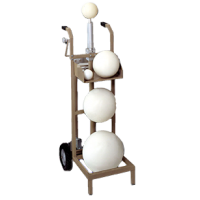
\includegraphics[width=\textwidth]{bss}
\caption{Bonner Sphere Spectrometer CITE}
\end{figure}
\end{column}
\begin{column}{.5\textwidth}
\begin{itemize}
\item Active detection through $^6$Li($n$, $\alpha$)T
\item Thermally sensitive crystal
\item Increasing HDPe sphere sizes provide different (faster) responses.
\end{itemize}
\end{column}
\end{columns}
\end{frame}

%%%%%%%%%%%%%%%%%%%%% gold foil based spectrometers
\begin{frame}
\frametitle{Foil-based Spectrometers}

\begin{itemize}
\item Passive detection through various reactions, [($n$, $\gamma$), ($n$, $\alpha$), etc.]
\item Secondary $\gamma$-ray actually what is measured
\item Multi-foil experiment can span entire spectrum
\item Gold (thermally sensitive) can be used in conjunction with Bonner Spheres
\end{itemize}

\end{frame}

%%%%%%%%%%%%%%%%%%%%% the mathematic formulation/unfolding
\begin{frame}
\frametitle{Problem Formulation}
\begin{equation}
\label{eqn:disc-response}
N_k + \epsilon_k = \sum_i R_{ki} \phi_i, \quad k = 1,\ldots, m .
\end{equation}

$N_k$ Measured response of detector $k$\\
$\epsilon_k$ (Unknown error) of detector $k$ response\\
$R_{ki}$ Response function of detector $k$ at energy $i$\\
$\phi_i$ Flux in energy $i$\\

\end{frame}


%%%%%%%%%%%%%%%%%%%%% doroshenko directed divergence
\begin{frame}
\frametitle{Doroshenko Directed Divergence}

\begin{equation}
\label{eqn:doroshenko}
\phi_j^{k + 1} = \phi_j^{k} (\frac{\sum_i \frac{R_{ji}}{\sum_j R_{ij} \phi_j^k}}{\sum_i \frac{R_{ji}}{N_i}}) 
\end{equation}

\end{frame}

%%%%%%%%%%%%%%%%%%%%% gravel/sandii
\begin{frame}
\frametitle{Gravel}

\begin{equation}
\label{eqn:sandii}
\phi_j^{k + 1} = \phi_j^{k} exp(\frac{\sum_i W_{ji}^k \log(\frac{N_i}{\sum_{j'} R_{ij'} \phi_{j'}^k})}{\sum_i W_{ji}^k}) ,
\end{equation}

\begin{equation}
\label{eqn:gravel-w}
W_{ji}^k = \frac{R_{ij} \phi_{j}^k}{\sum_{j'} R_{ij'} \phi_{j'}^k} \frac{N_i^2}{\sigma_i^2} ,
\end{equation}
\end{frame}

%%%%%%%%%%%%%%%%%%%%% maxed
\begin{frame}
\frametitle{MAXED}
\begin{equation}
\label{eqn:maxed-skilling}
S = - \sum [\phi_j \ln (\frac{\phi_j}{\phi_j^{DEF}}) + \phi_j^{DEF} - \phi_j]
\end{equation}
\end{frame}


%%% NEBP Modeling Effort (10) ---------------------------------------------------------------------------------------
\section{Simulated Work}
%%%%%%%%%%%%%%%%%%%%% modeling steps/overview
\begin{frame}
\frametitle{Modeling Overview}

\begin{itemize}
\item Added NEBP to existing model
\item Tallied fission rates within core to produce SDEF
\item Applied ADVANTG variance reduction software to speedup tally convergence
\item Tallied flux at NEBP aperture
\end{itemize}

\end{frame}

%%%%%%%%%%%%%%%%%%%%% existing model
\begin{frame}
\frametitle{Existing Model}

\begin{figure}
\centering
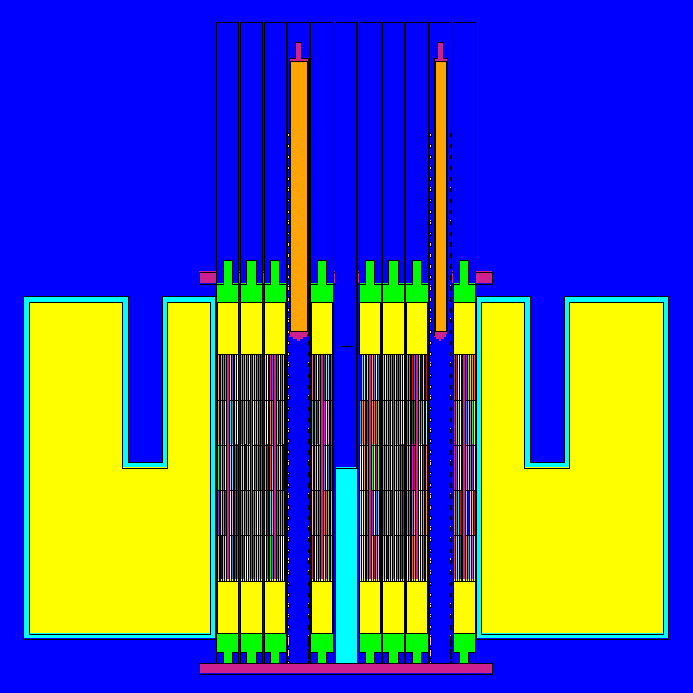
\includegraphics[width = .5\textwidth]{existingyz}
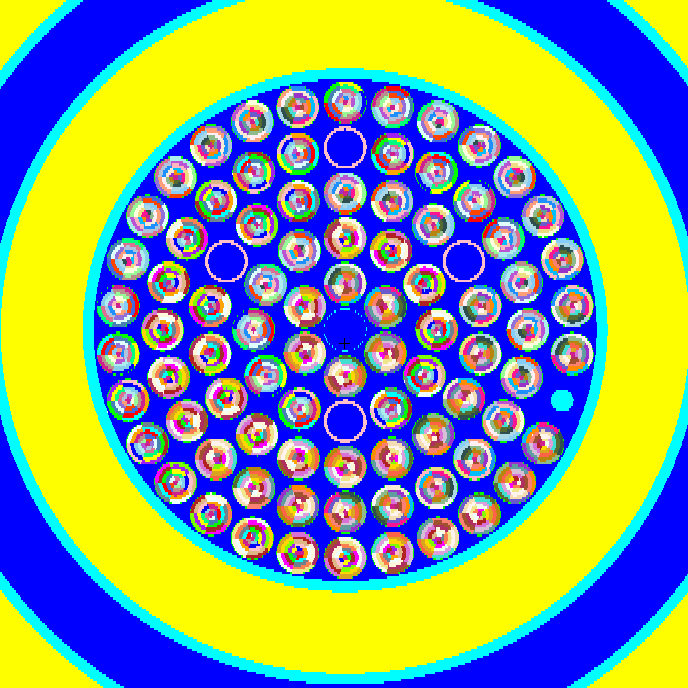
\includegraphics[width = .5\textwidth]{existingxy}
\caption{YZ (left) and XY (right) views of the existing core model with discretized fuel, control rods, graphite reflector, etc.}
\end{figure}

\end{frame}

%%%%%%%%%%%%%%%%%%%%% nebp additions
\begin{frame}
\frametitle{NEBP Additions}

\begin{figure}
\centering
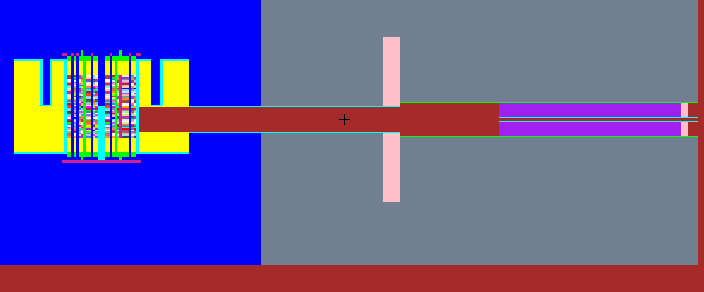
\includegraphics[trim=0 40 0 20, clip, width = .9\textwidth]{mcnp_newxz}\\
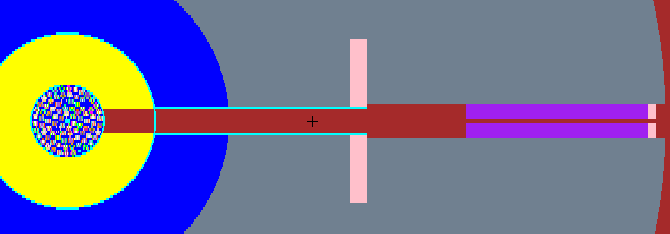
\includegraphics[trim=0 120 0 120, clip, width = .9\textwidth]{mcnp_newxy}
\caption{XZ (top) and XY (bottom) views of the NEBP additions with reflector penetration, lead shadow shield, and collimator.}
\end{figure}

\end{frame}

%%%%%%%%%%%%%%%%%%%%% fission tally results I
\begin{frame}
\frametitle{Fission Tally Results}

\begin{columns}[c]
\begin{column}{.5\textwidth}
\begin{figure}
\centering
Example results from fission tallies within core fuel, B-ring radial (left), fuel element slice (middle), F-ring axial (right).
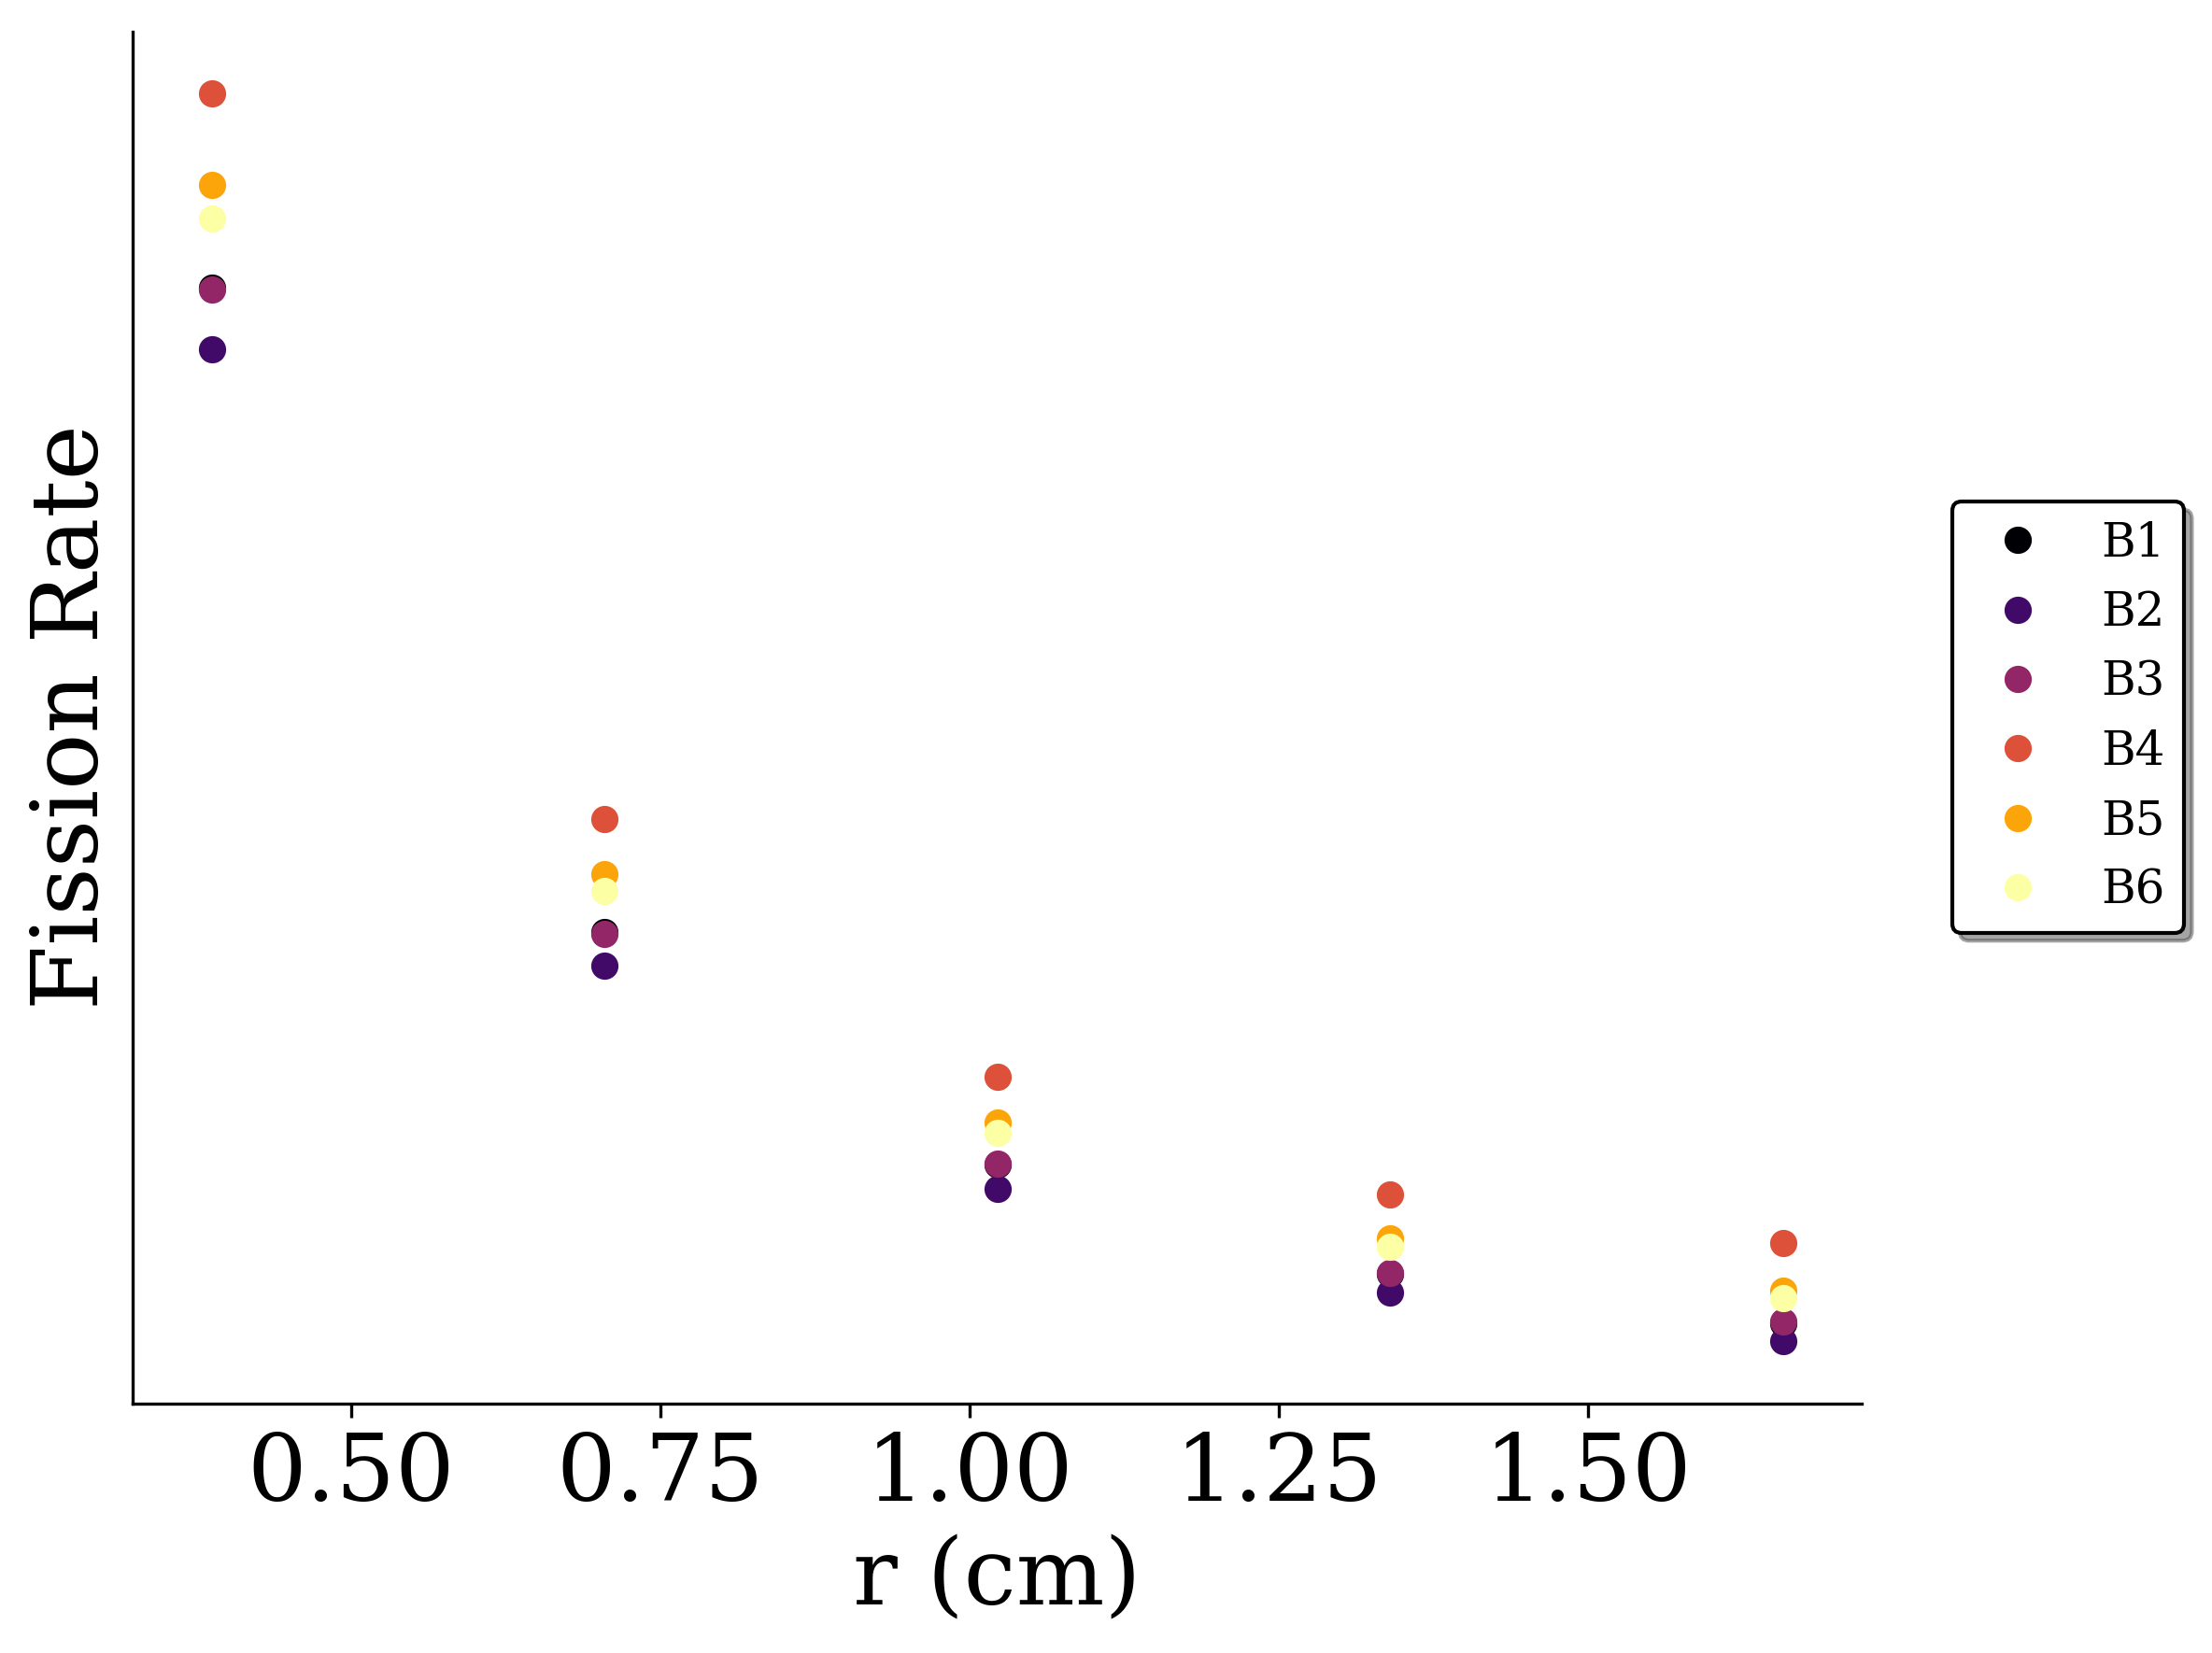
\includegraphics[width = 1.0\textwidth]{radial_rr_density_B}
\end{figure}
\end{column}
\begin{column}{.5\textwidth}
\begin{figure}
\centering
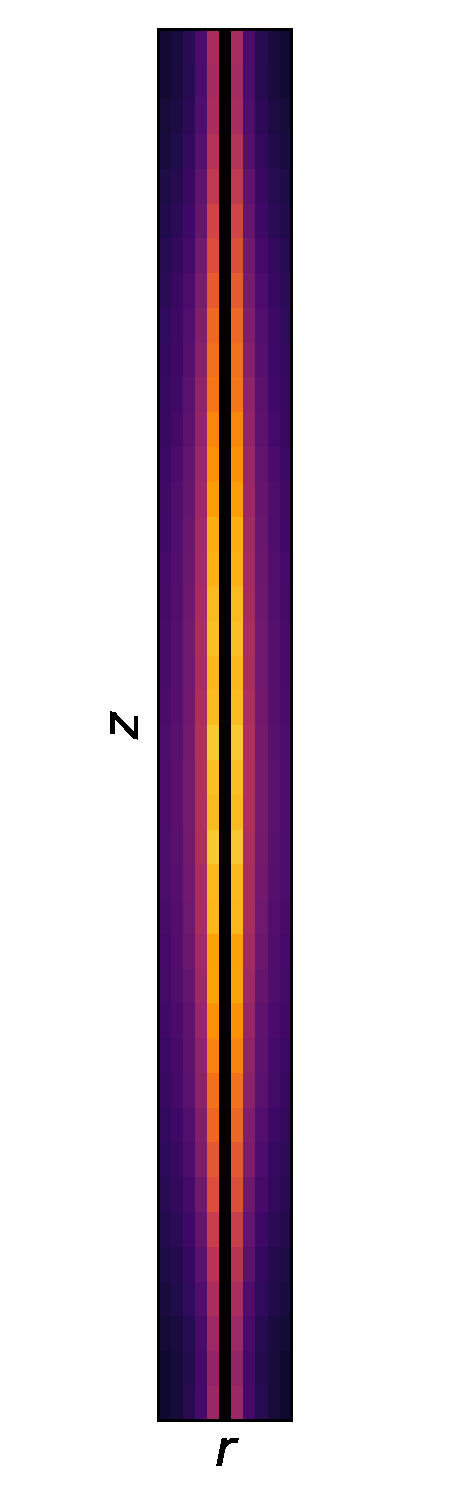
\includegraphics[height = 0.8\textheight]{rr_dist_B1}
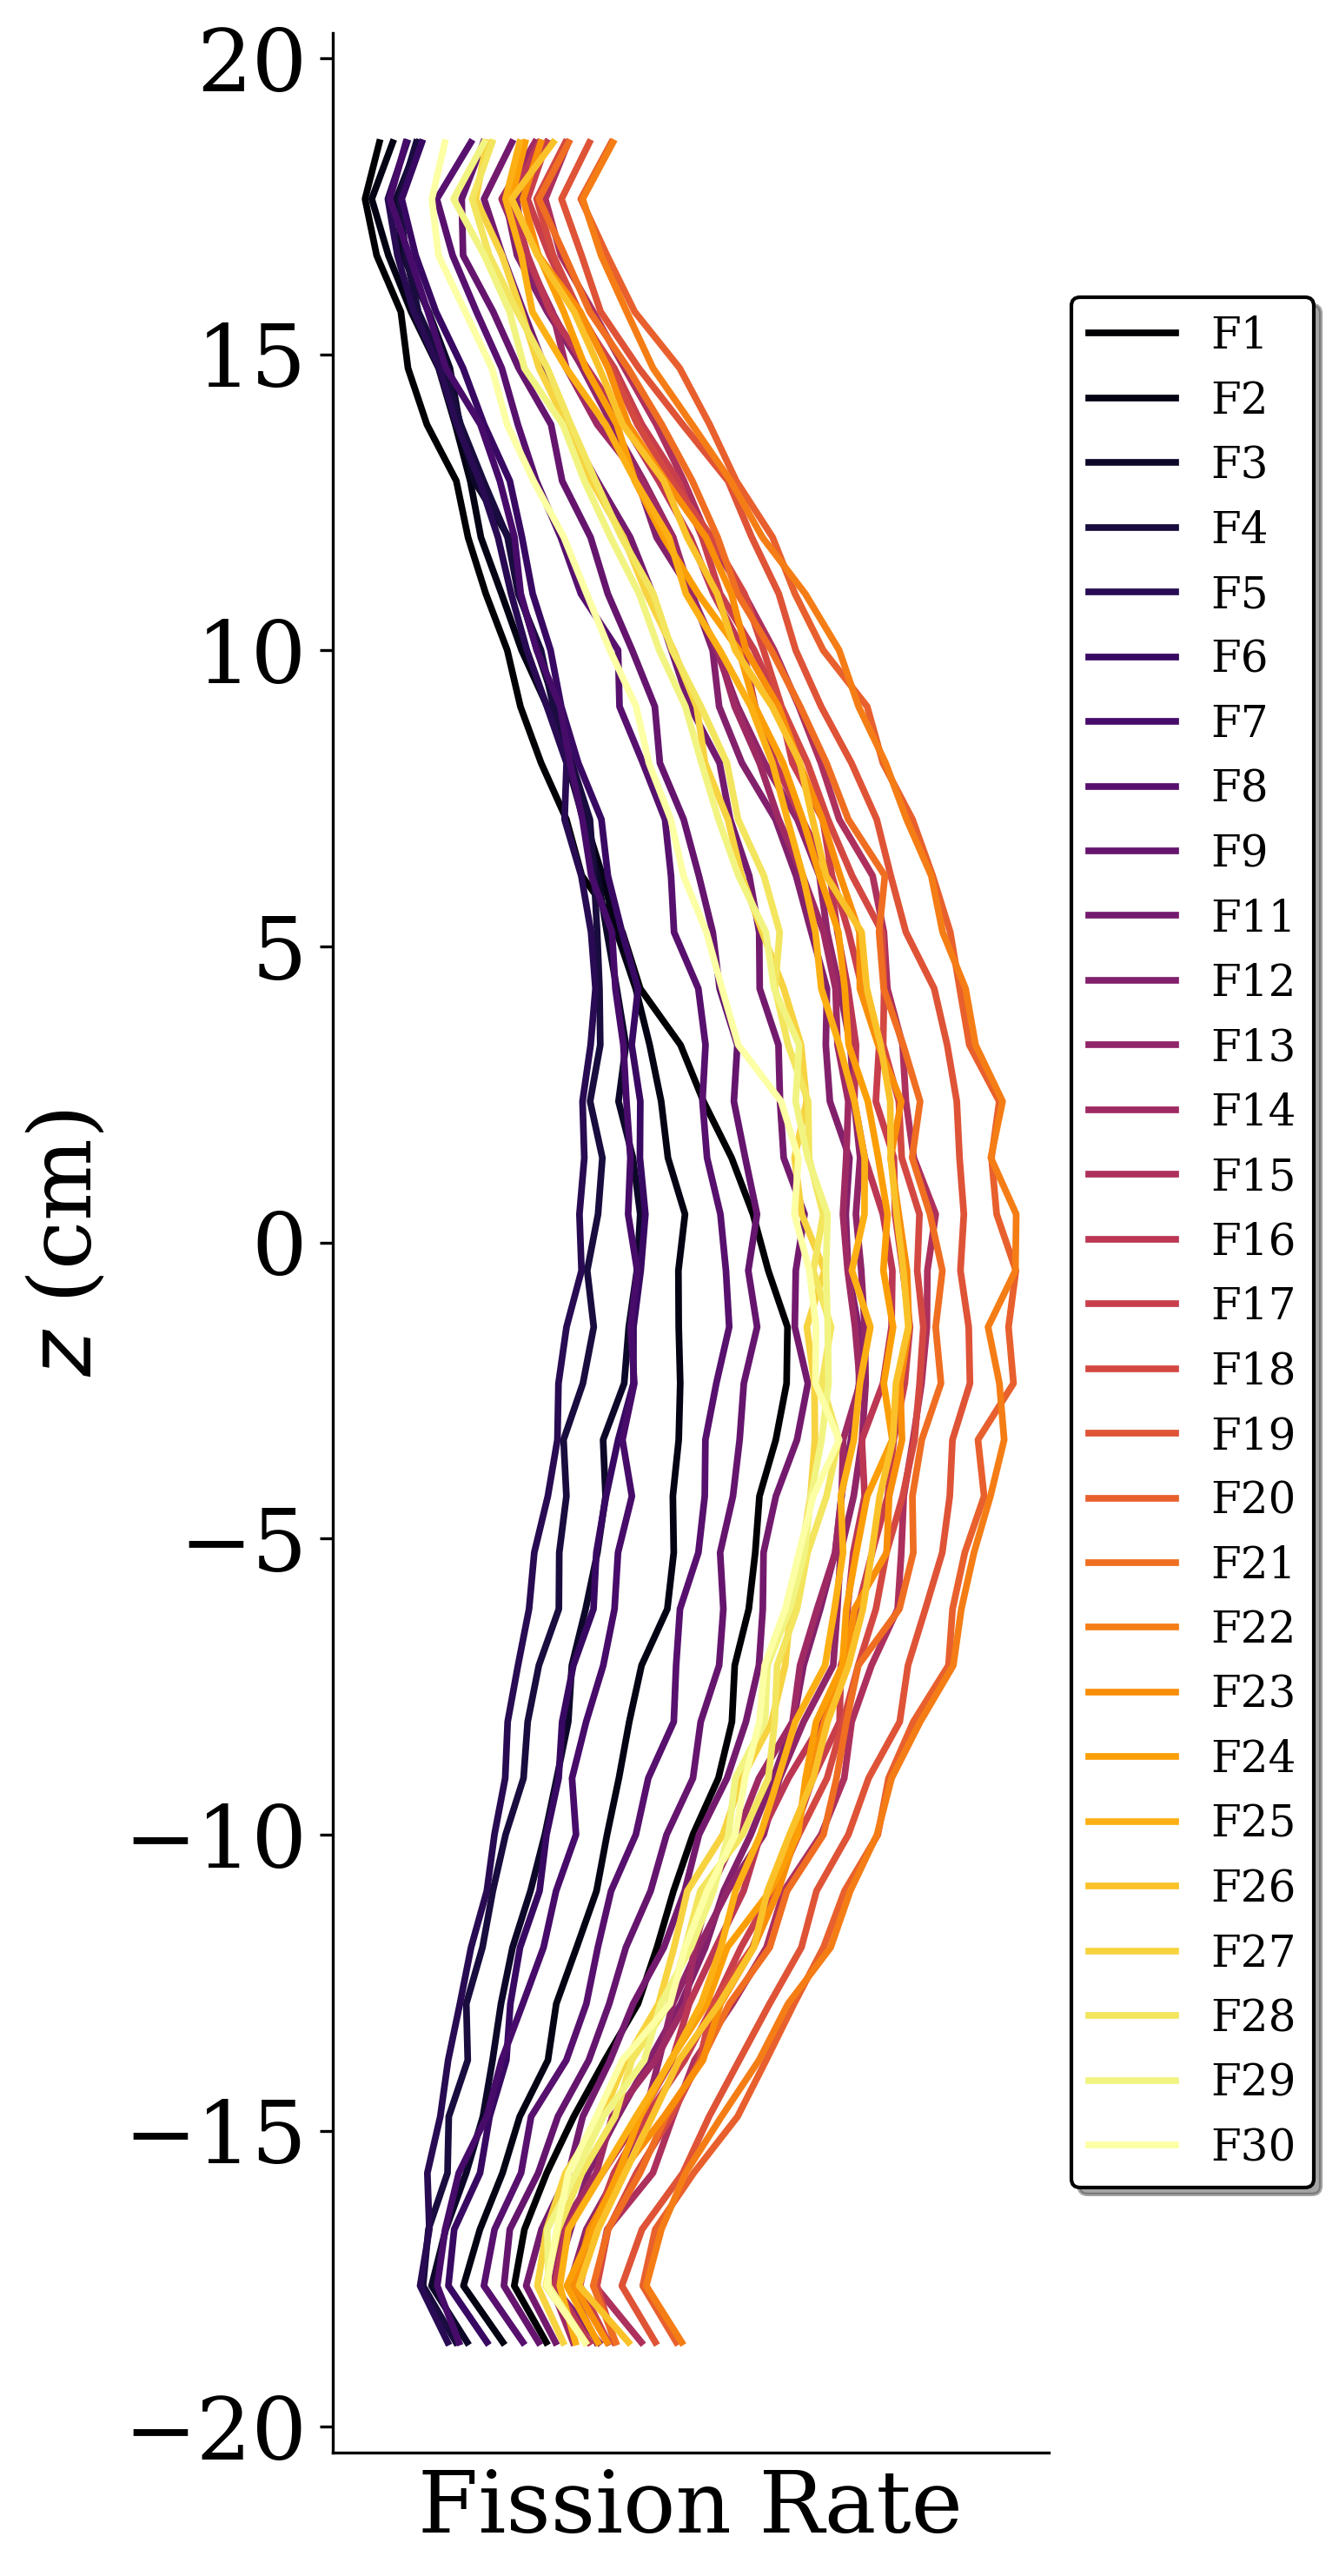
\includegraphics[height = 0.8\textheight]{axial_rr_density_F}
\end{figure}
\end{column}
\end{columns}

\end{frame}

%%%%%%%%%%%%%%%%%%%%% fission tally results II
\begin{frame}
\frametitle{Fission Tally Results}

\begin{figure}
\centering
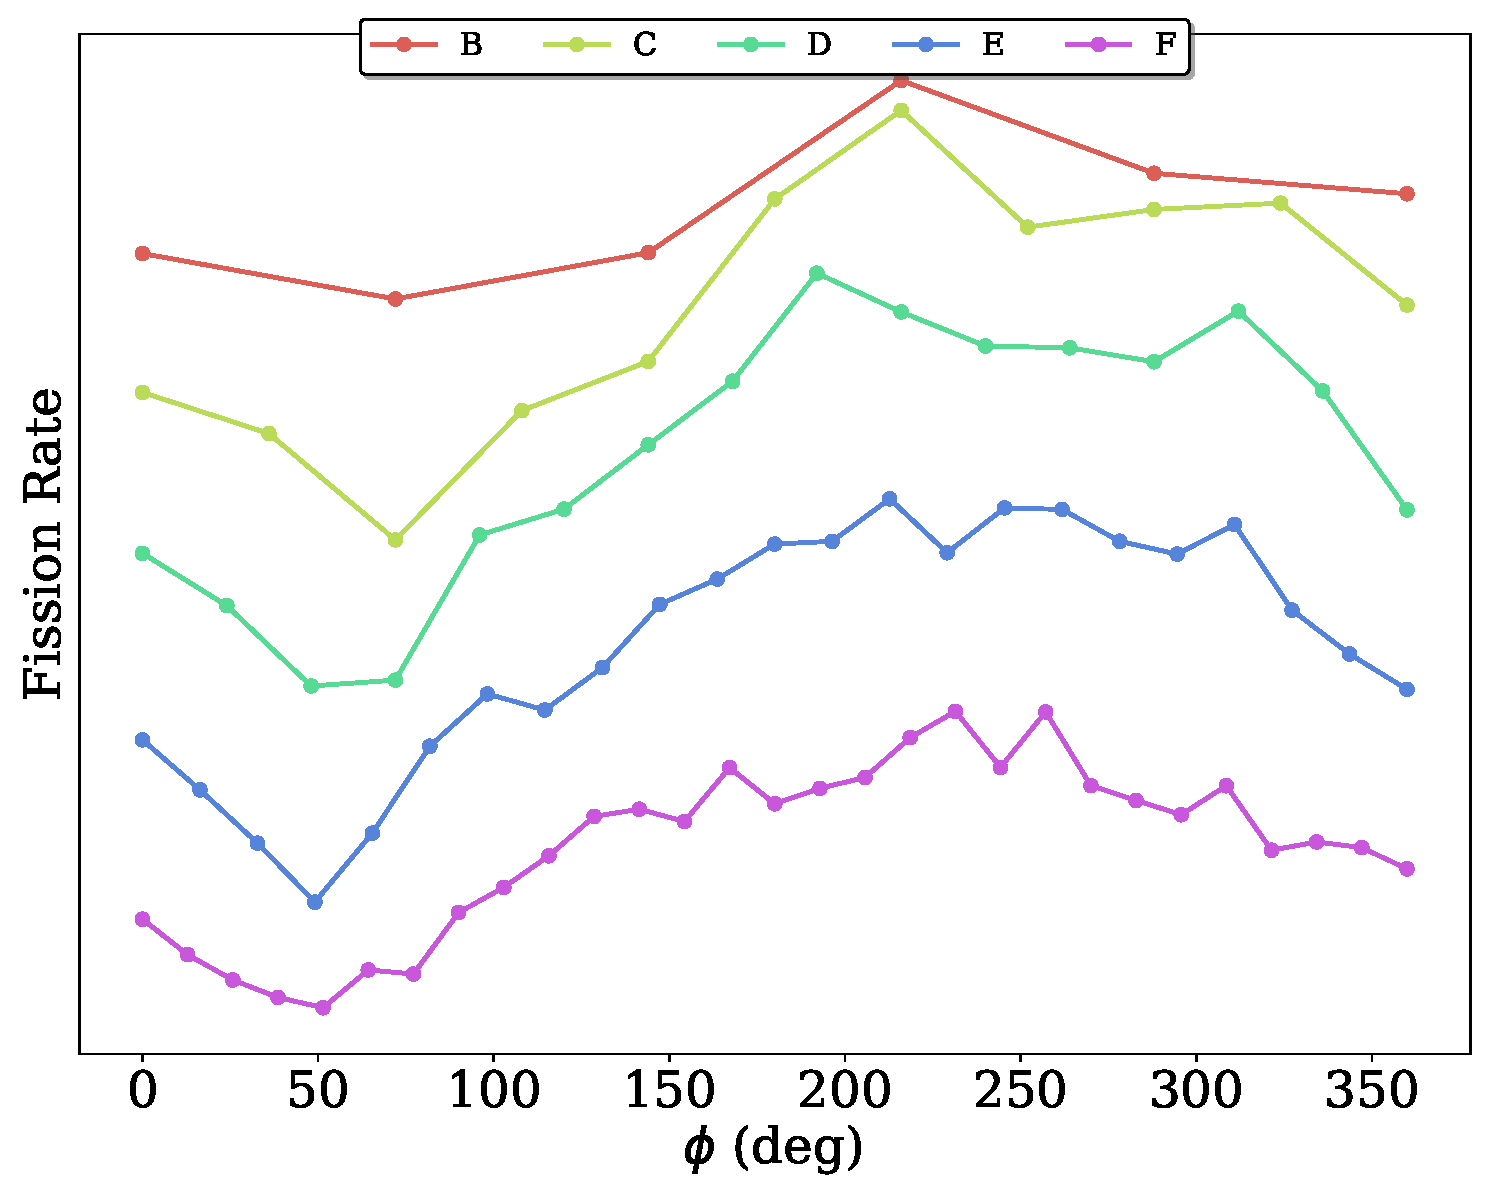
\includegraphics[width = 0.7\textwidth]{totals_azi}
\caption{}
\end{figure}

\end{frame}

%%%%%%%%%%%%%%%%%%%%% applyting advantg
\begin{frame}
\frametitle{Applying ADVANTG}

\begin{table}[h]\centering
\label{tab:advantg_params}
\caption{Input parameters used for ADVANTG.}
\begin{tabular}{ r | l }
\toprule
model                     &   mcnp\\
method                    &   cadis\\
outputs                   &   mcnp\\
mcnp\_input               &   ksun.inp\\
mcnp\_tallies             &   11\\
mesh\_refinement          &   mcnp\\
mesh\_x                   &   -55 -22 22 184 368\\
mesh\_y                   &   -55 -22 -12 -2 2 12 22 55\\
mesh\_z                   &   -35 -16 -11 -5 0 35\\
mesh\_x\_ints             &   17 25 25 25\\
mesh\_y\_ints             &   75 14 17 22 17 14 17\\
mesh\_z\_ints             &   17 14 35 14 17\\
anisn\_library            &   bplus\\
denovo\_pn\_order         &   4\\
denovo\_quad\_num\_azi    &   15\\
denovo\_quad\_num\_polar  &   12\\
denovo\_x\_blocks         &   8\\
denovo\_y\_blocks         &   8\\
denovo\_z\_blocks         &   1\\
\end{tabular}
\end{table}

\end{frame}

%%%%%%%%%%%%%%%%%%%%% notes on speedup/runtime/cores,etc.
\begin{frame}
\frametitle{Runtime, speedup, etc.}

It sped up.

\end{frame}

%%%%%%%%%%%%%%%%%%%%% energy distribution
\begin{frame}
\frametitle{Spectral Flux}

\begin{figure}
\centering
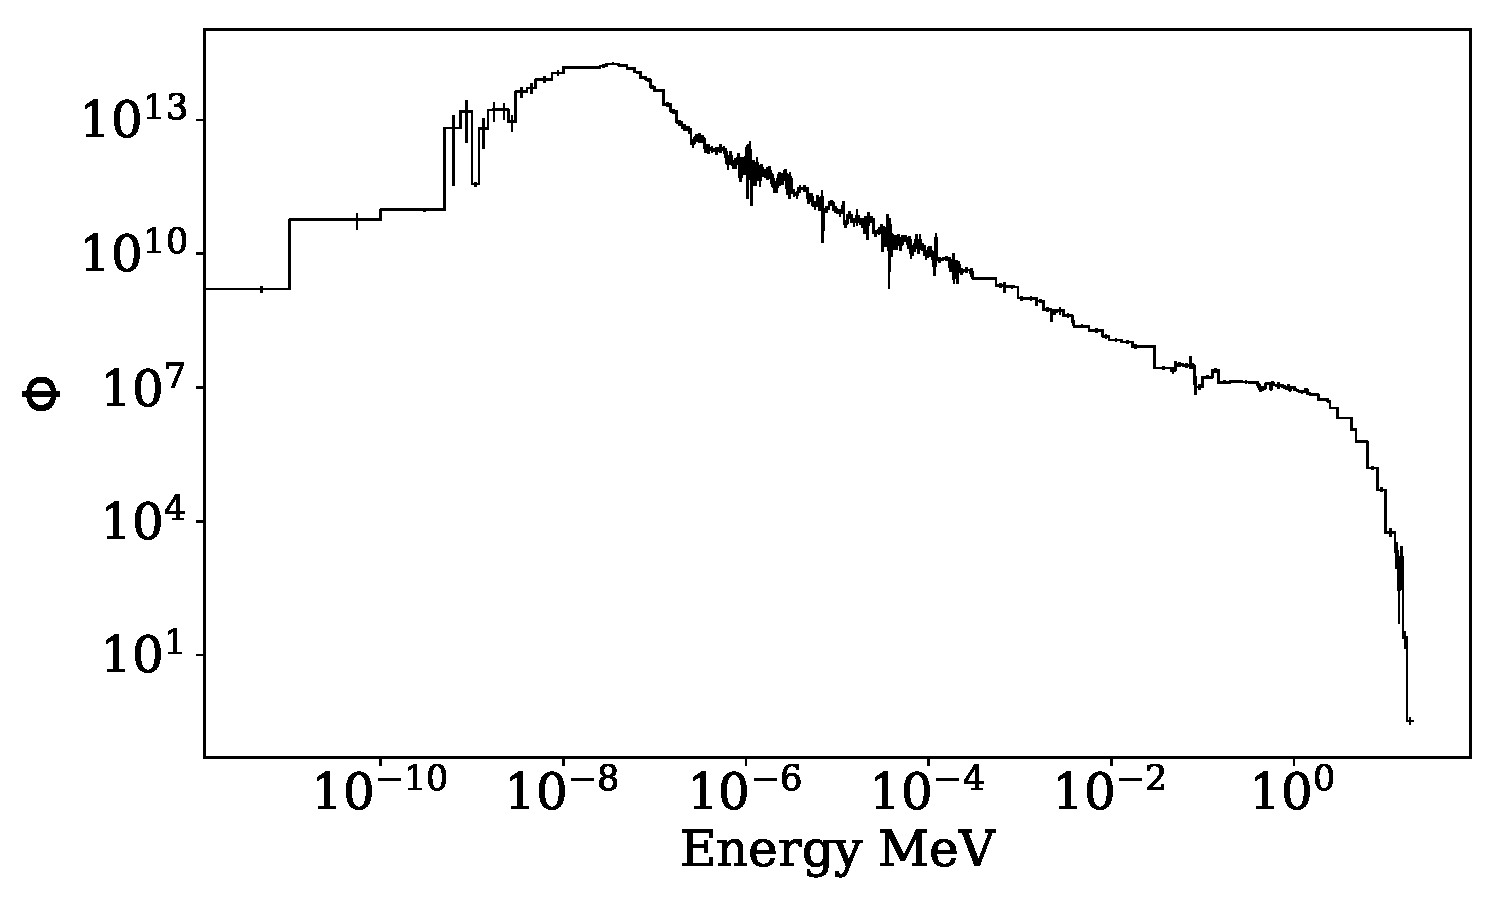
\includegraphics[width = 0.5\textwidth]{flux_erg}
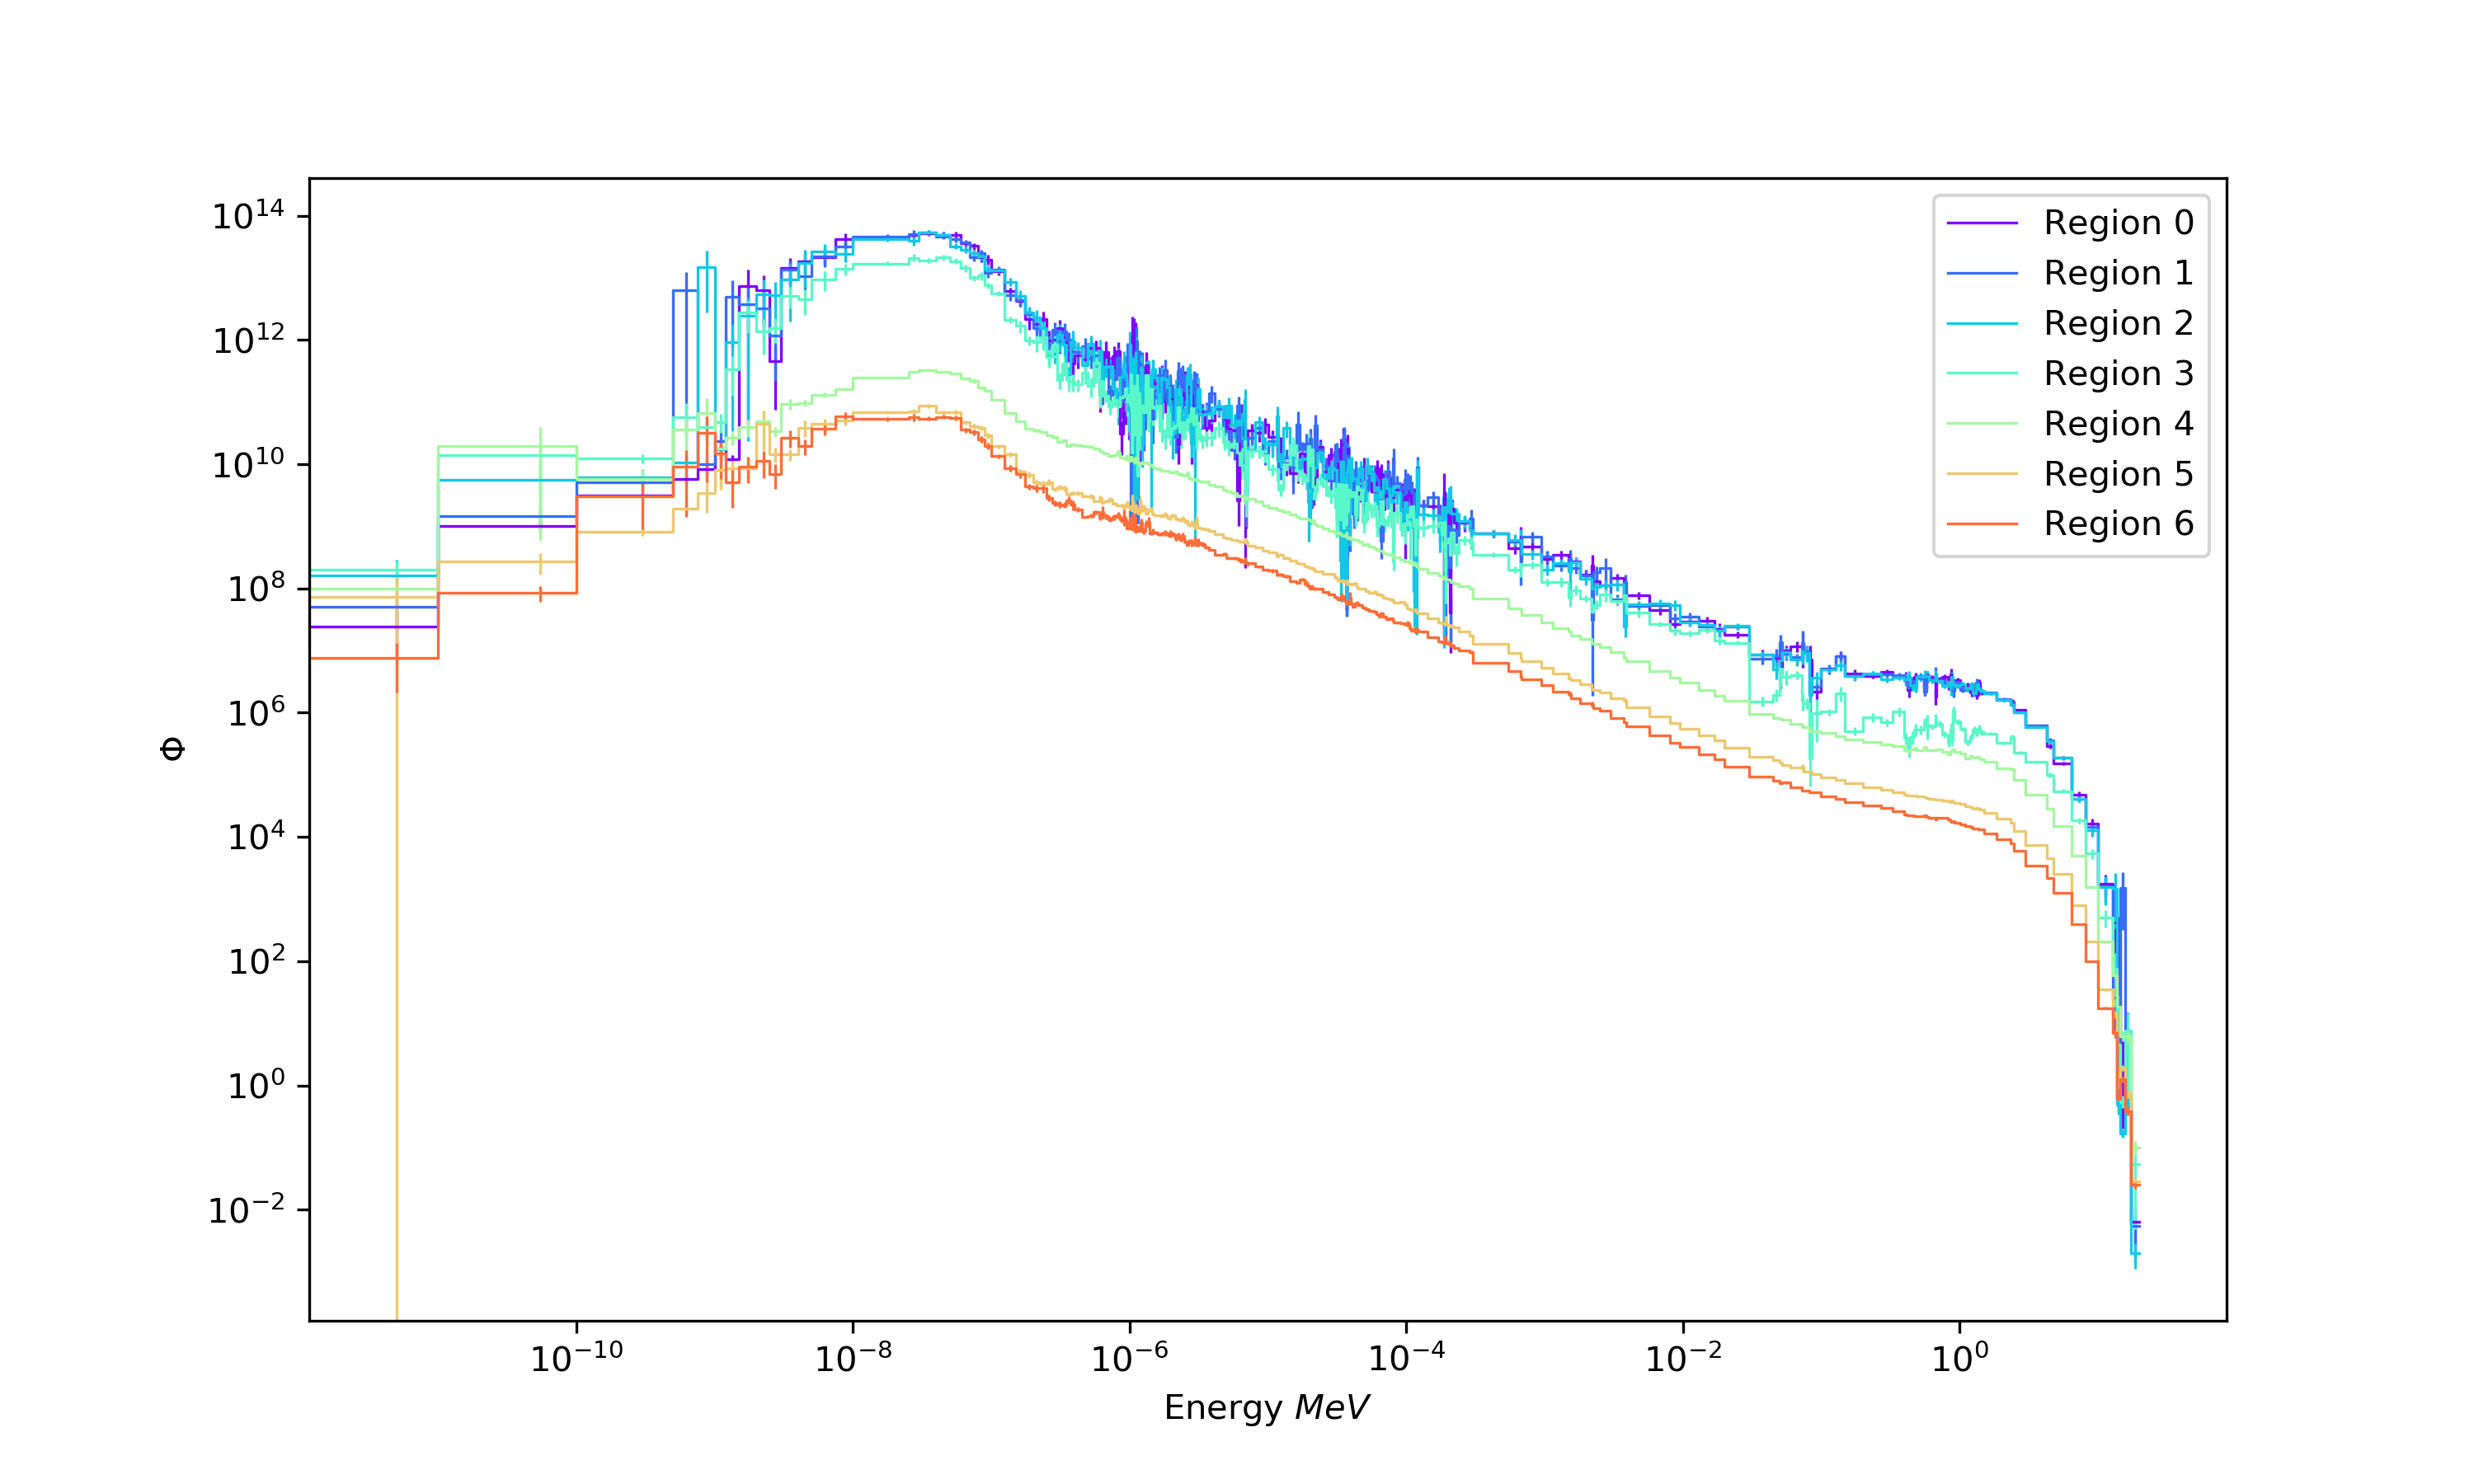
\includegraphics[width = 0.5\textwidth]{flux_rad_erg}
\caption{}
\end{figure}

\end{frame}

%%%%%%%%%%%%%%%%%%%%% cosine distribution
\begin{frame}
\frametitle{Angular Flux}

\begin{figure}
\centering
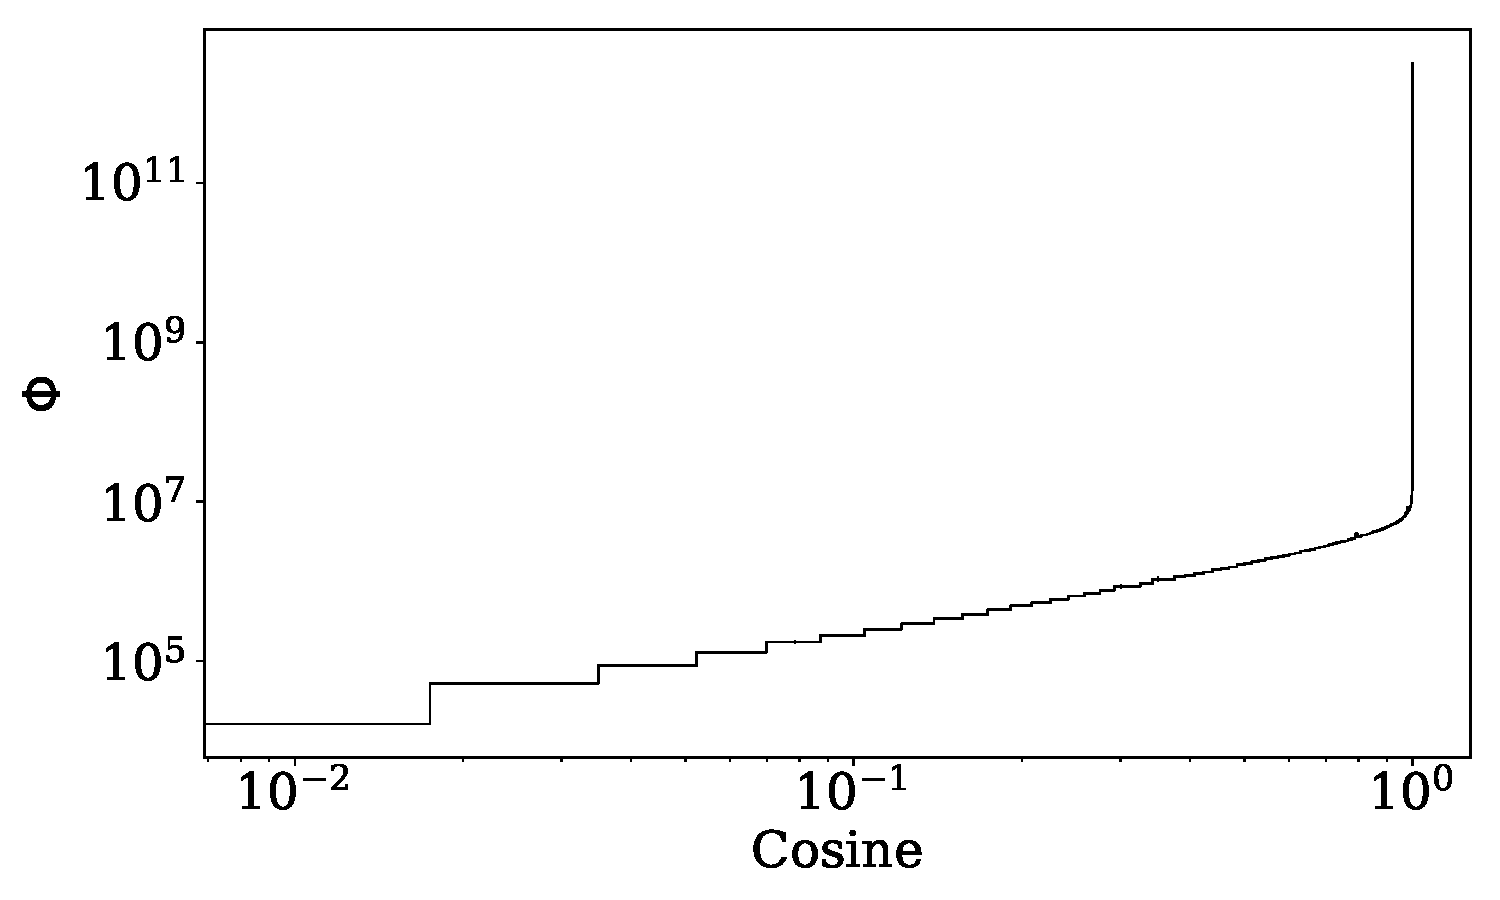
\includegraphics[width = 0.5\textwidth]{flux_cos}
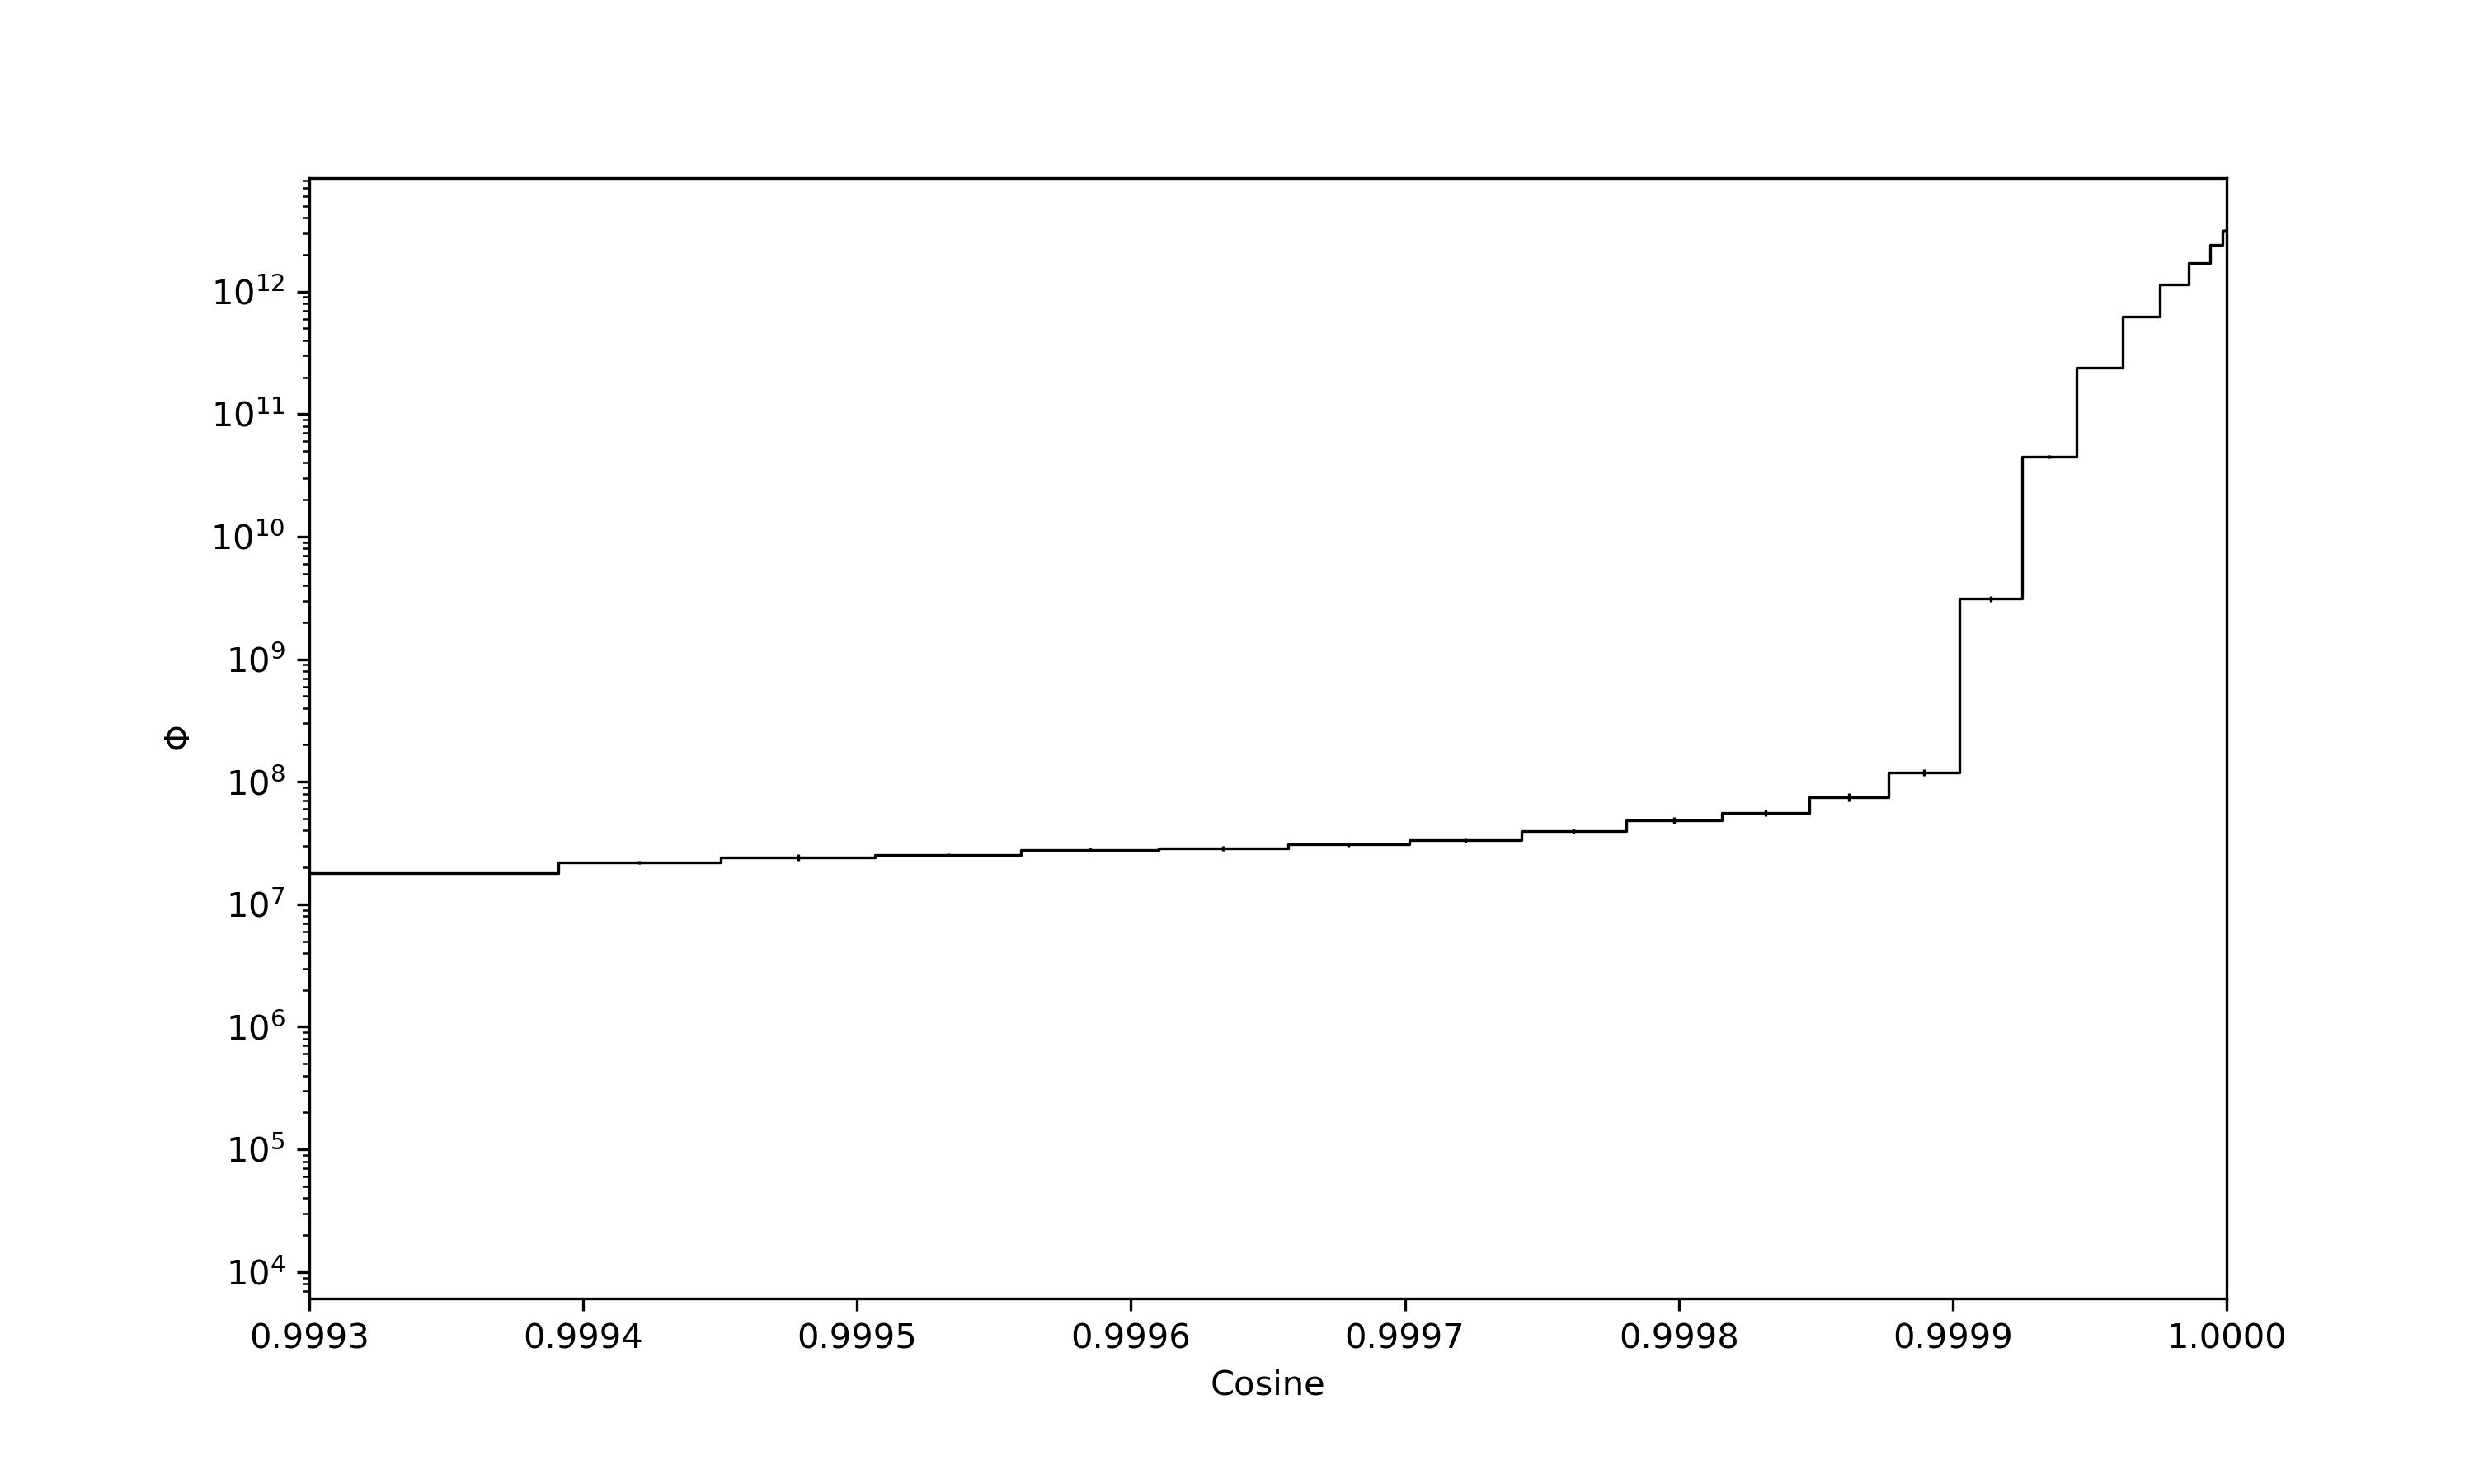
\includegraphics[width = 0.5\textwidth]{flux_cos_detail}
\caption{}
\end{figure}

\end{frame}

\begin{frame}
\frametitle{Angular Flux}

\begin{figure}
\centering
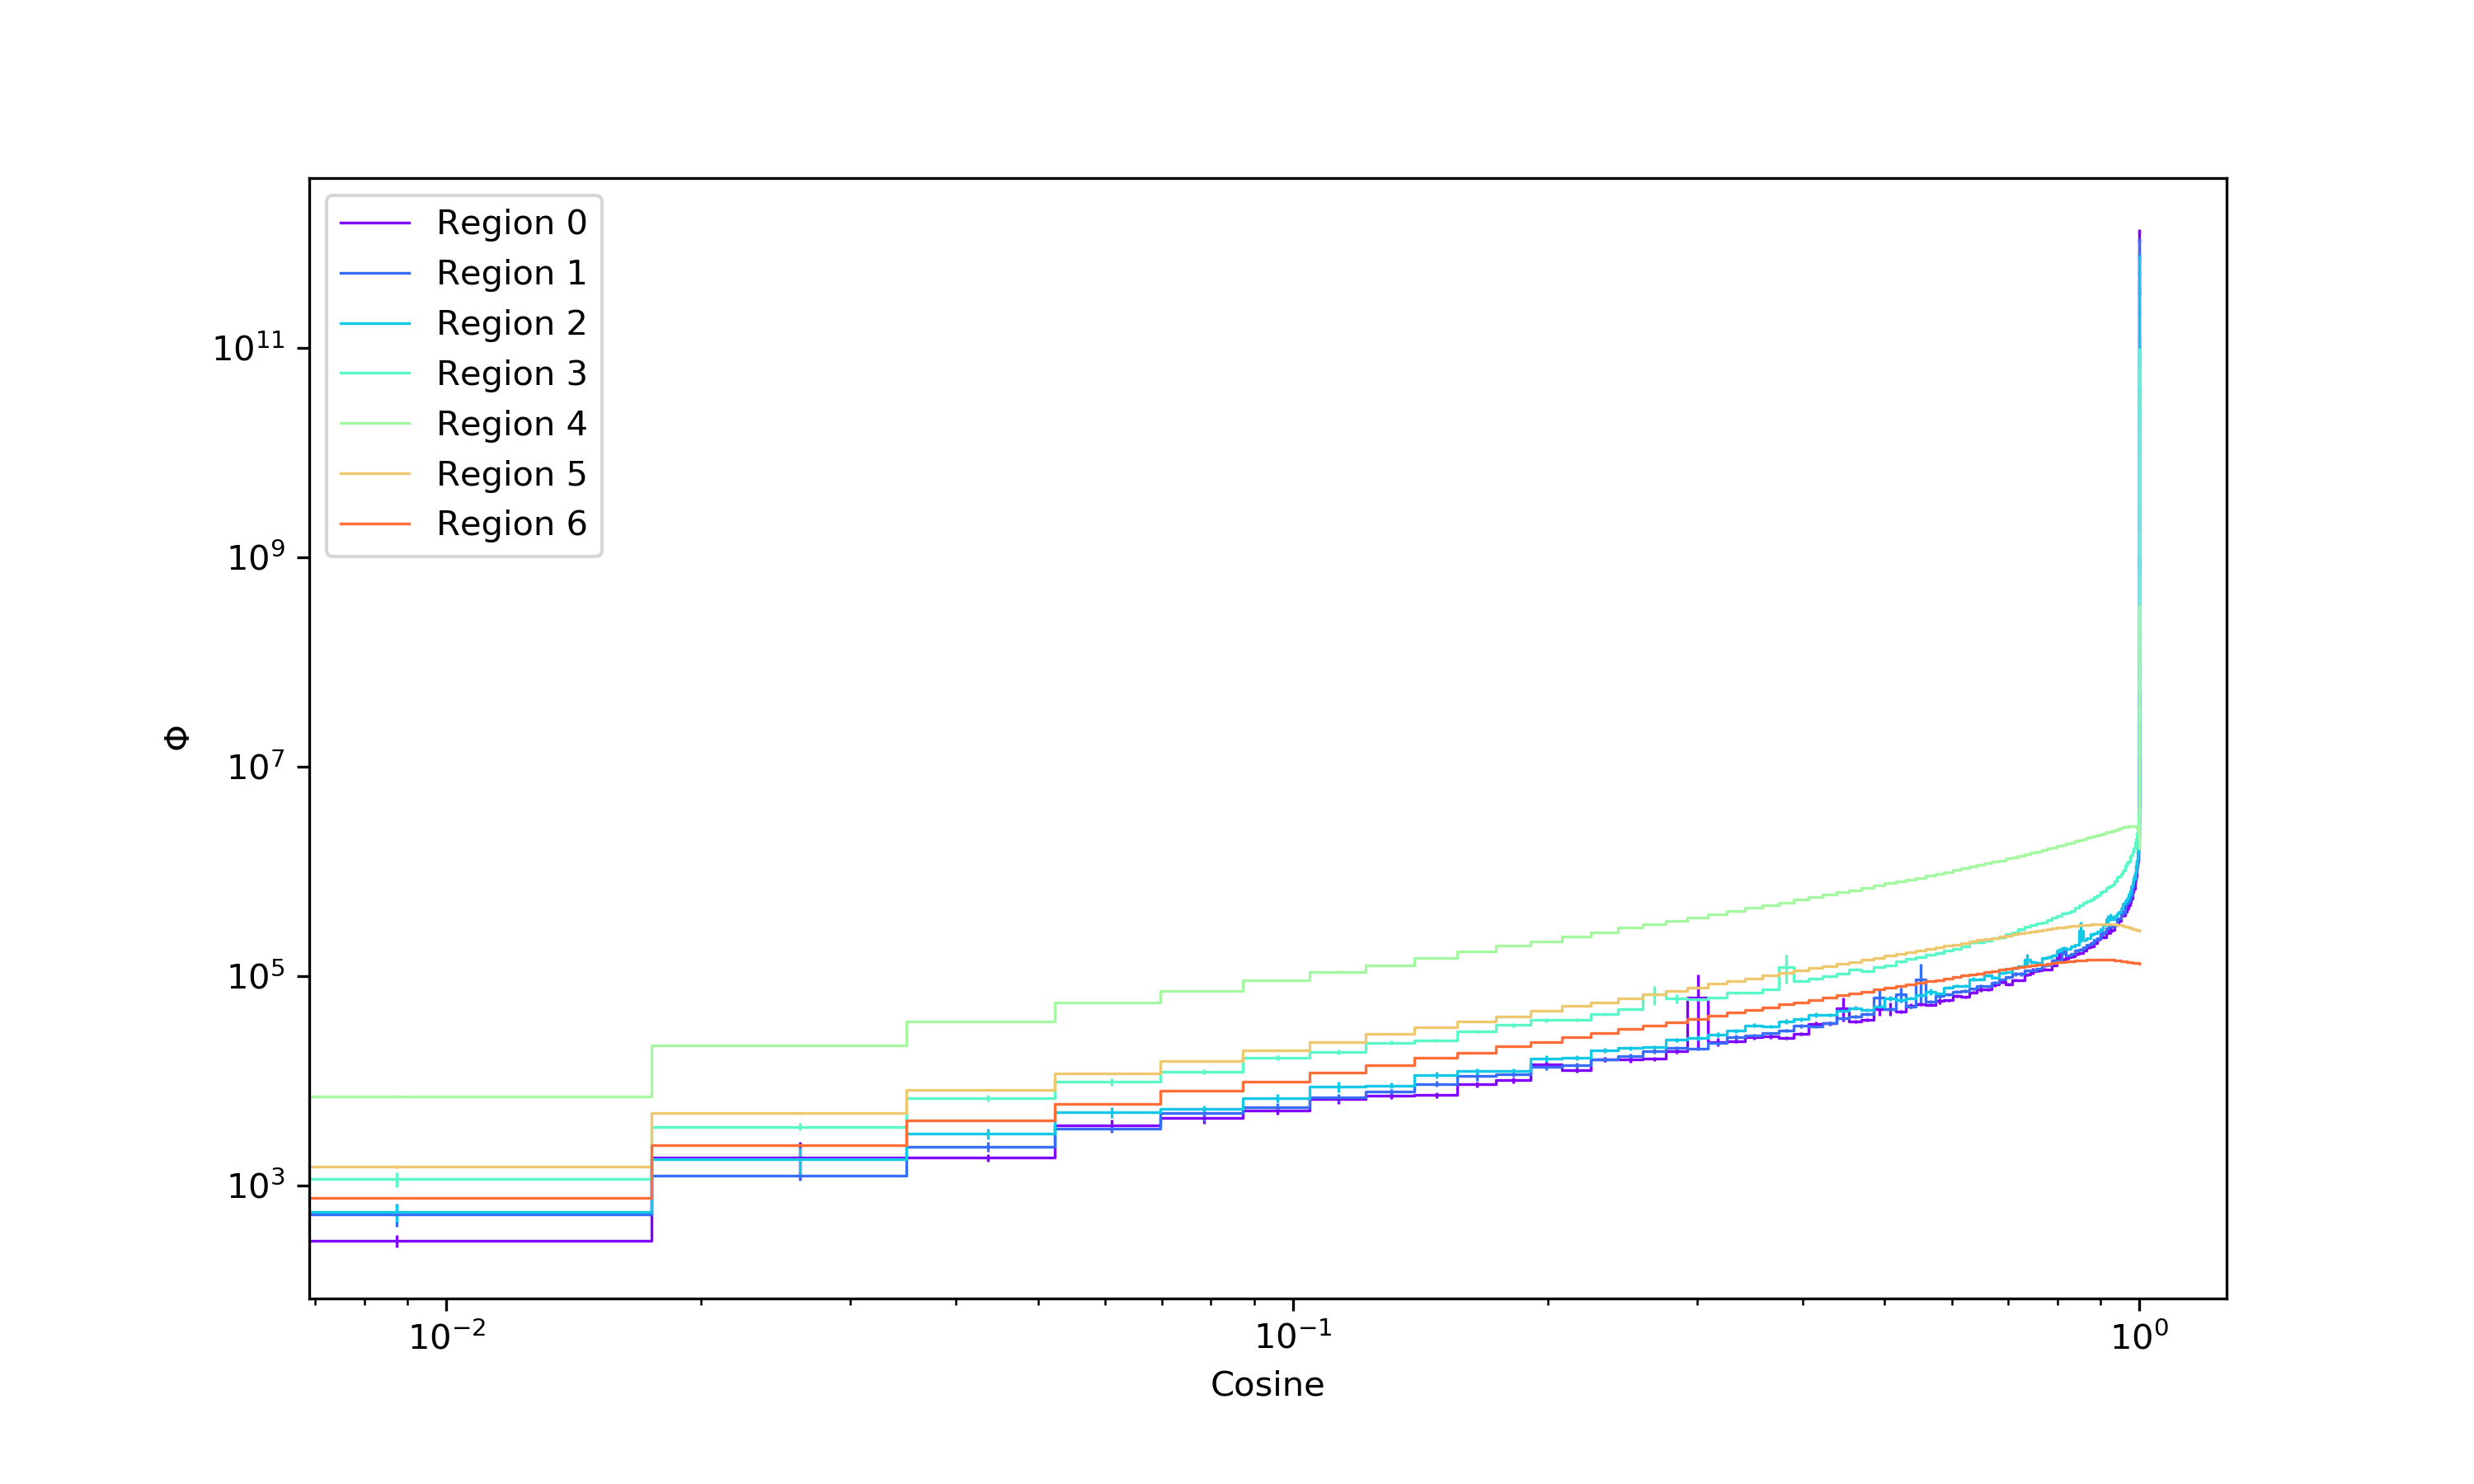
\includegraphics[width = 0.5\textwidth]{flux_rad_cos}
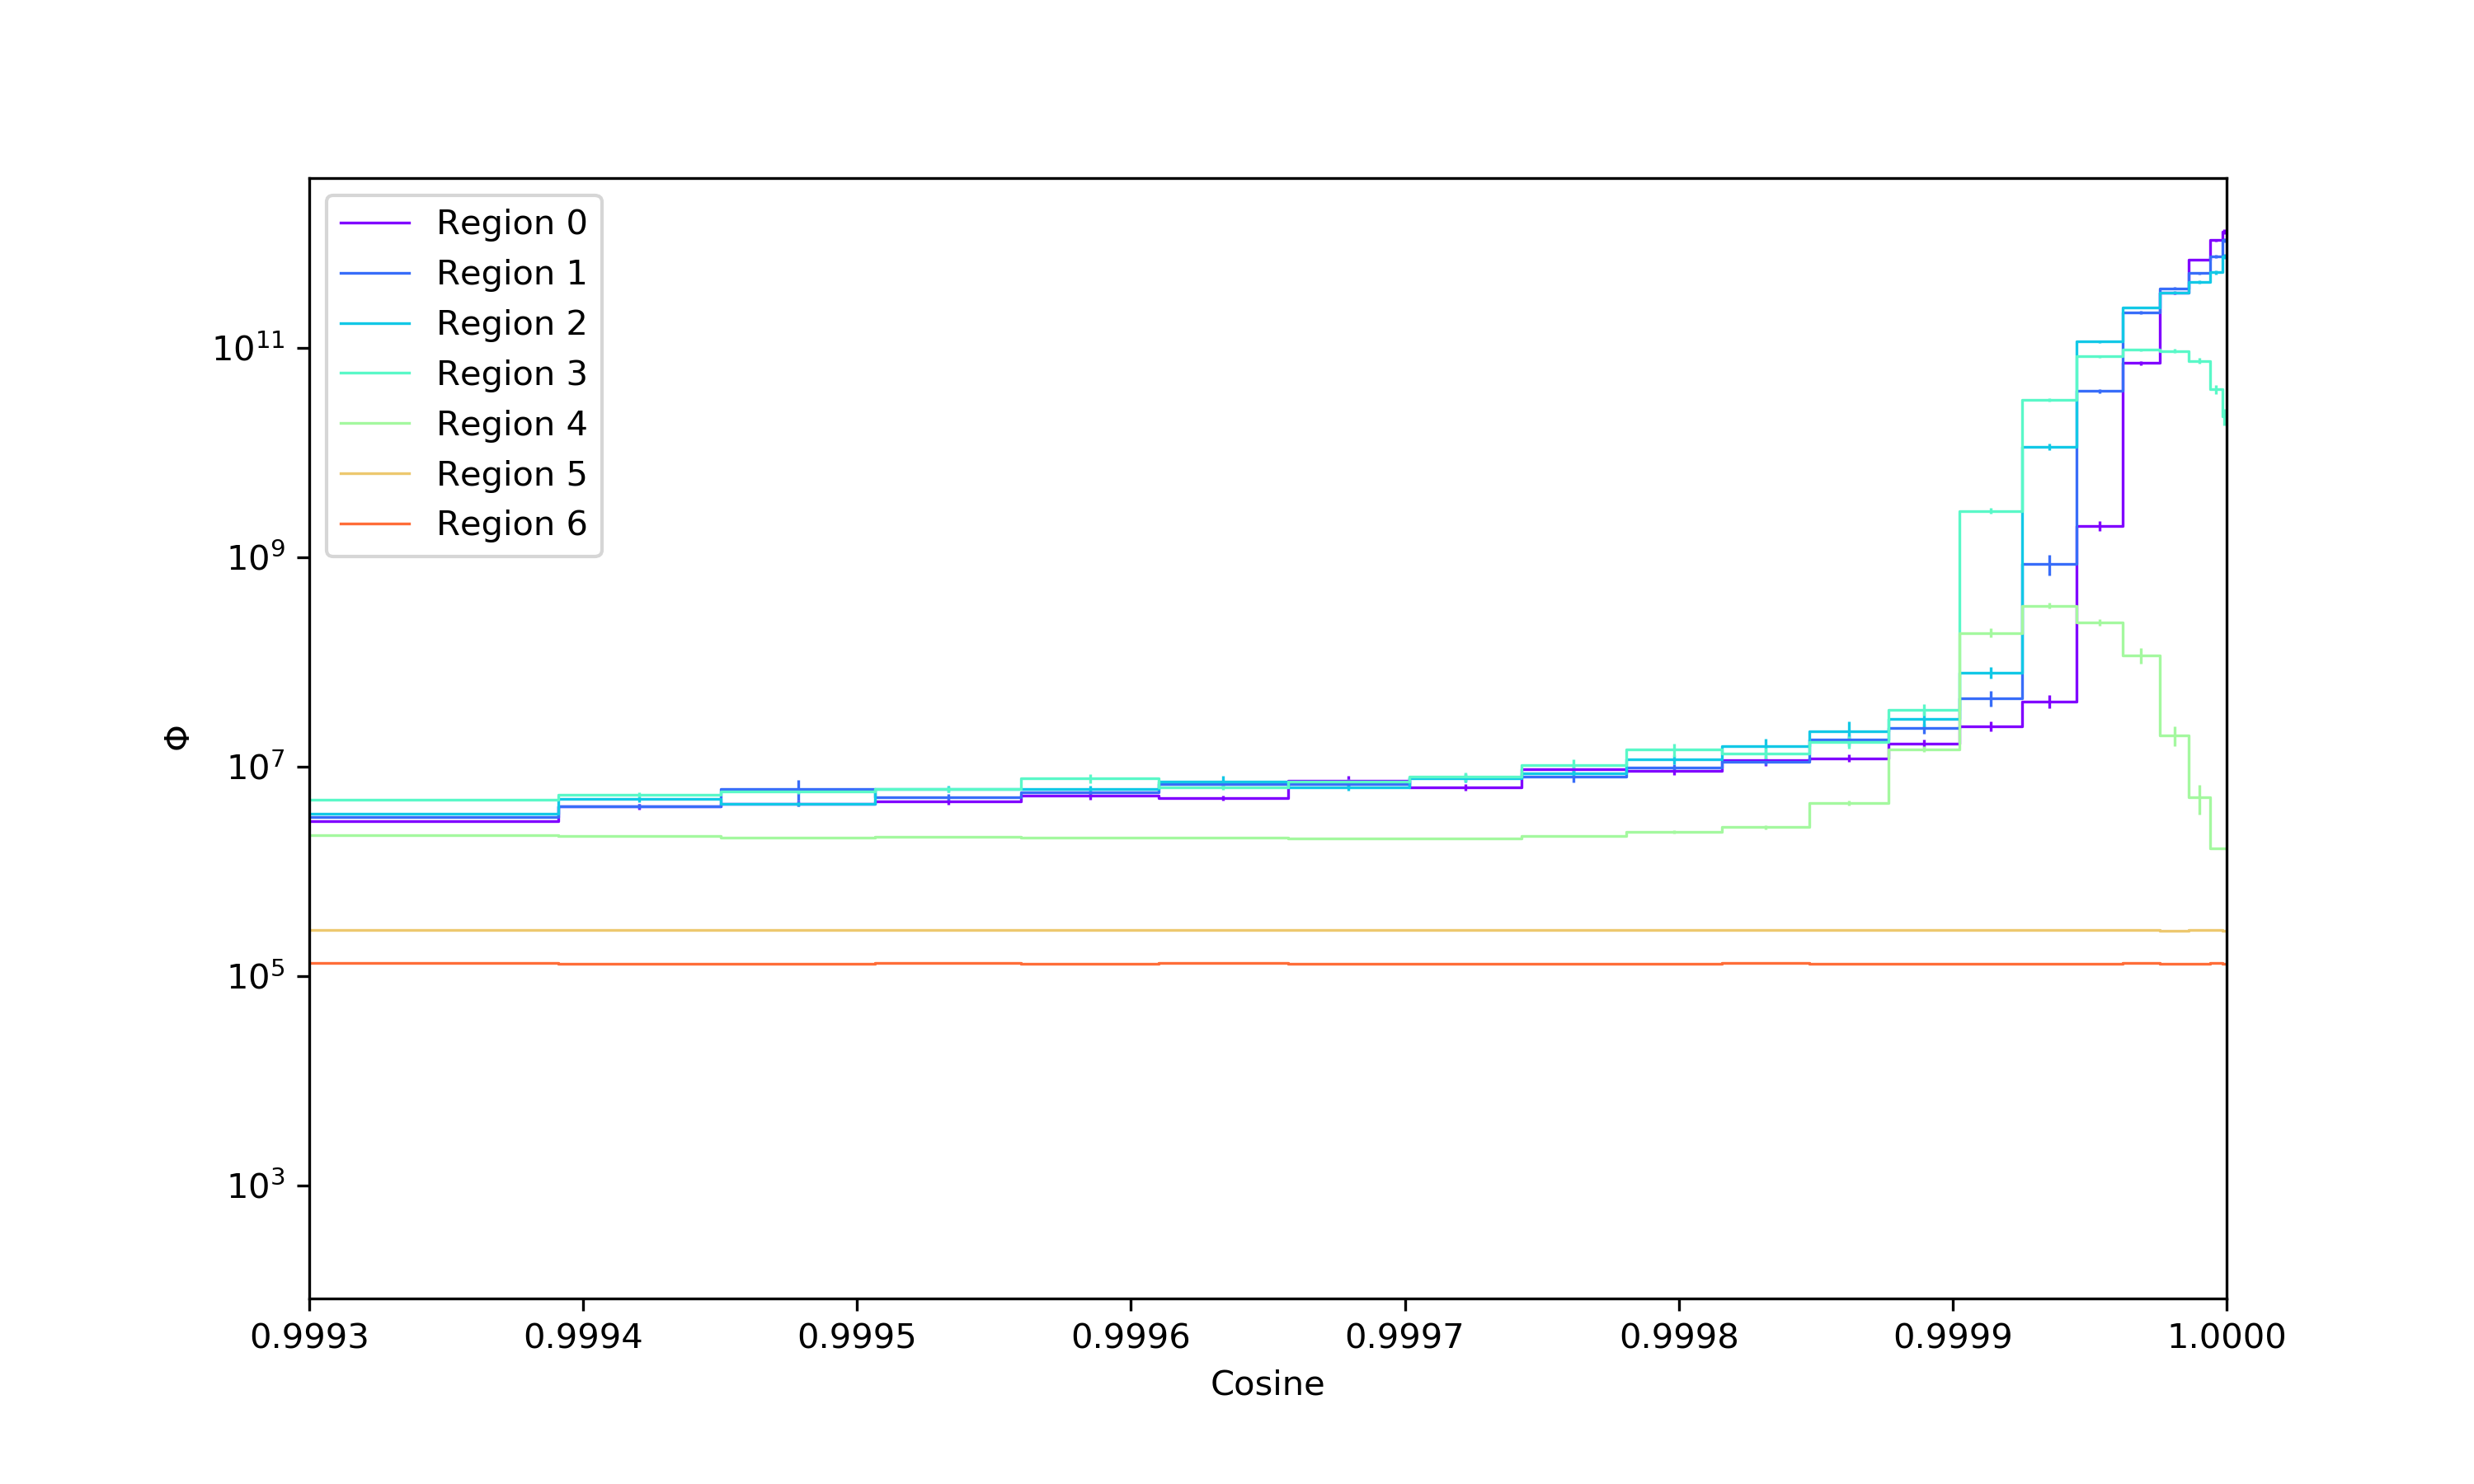
\includegraphics[width = 0.5\textwidth]{flux_rad_cos_detail}
\caption{}
\end{figure}

\end{frame}

%%%%%%%%%%%%%%%%%%%%% radial distribution
\begin{frame}
\frametitle{Radial Flux}

\begin{figure}
\centering
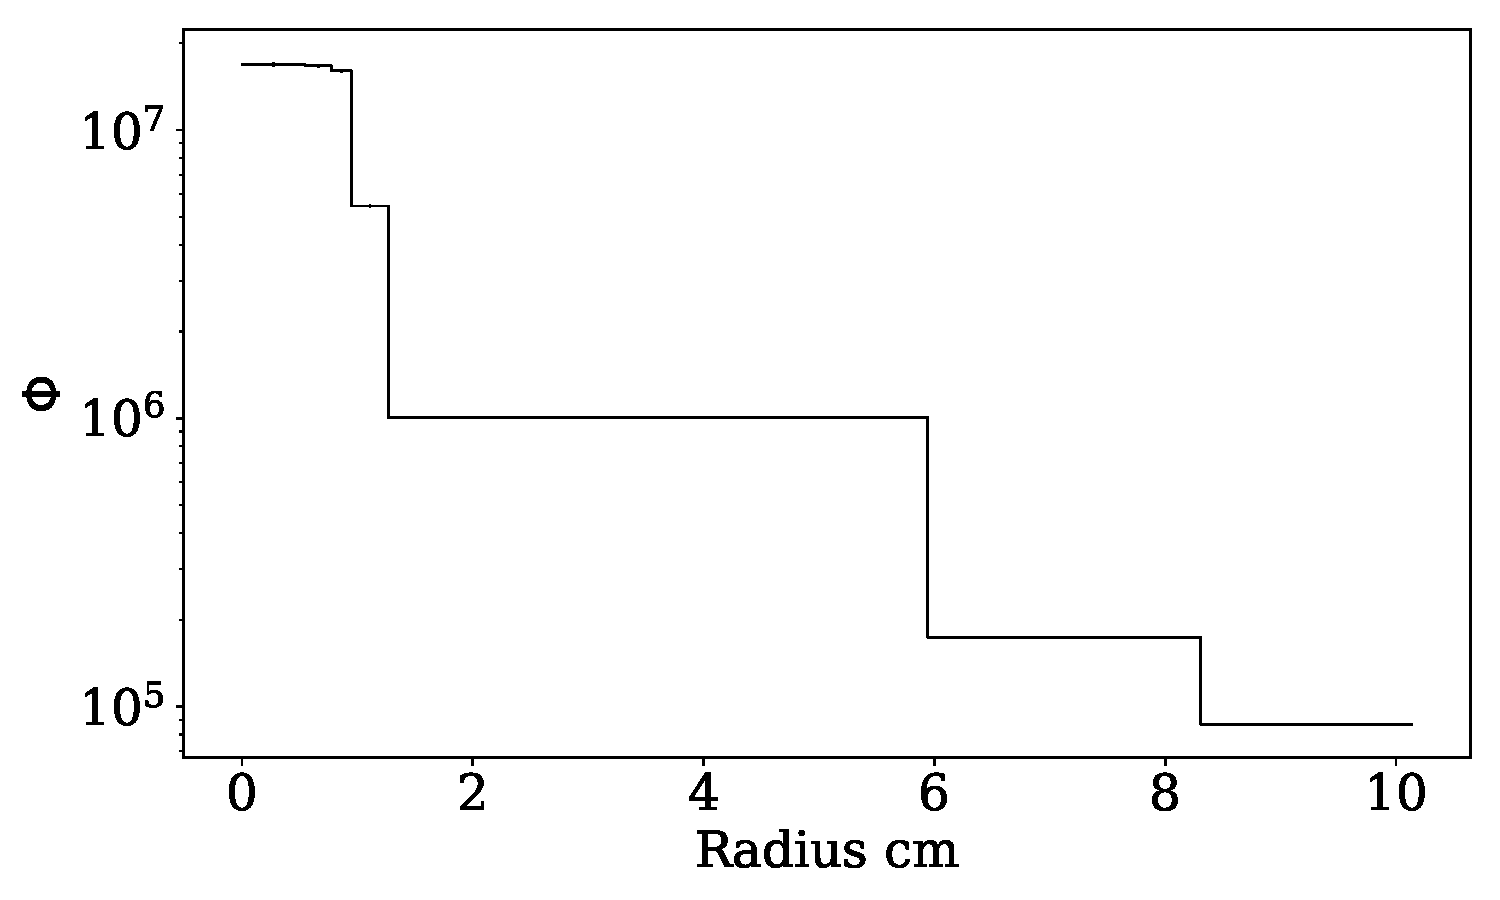
\includegraphics[width = 0.8\textwidth]{flux_rad}
\caption{}
\end{figure}

\end{frame}

%%% NEBP Experimental Campaign (14) ---------------------------------------------------------------------------------------
\section{Experimental Work}
%%%%%%%%%%%%%%%%%%%%% modeling steps
\begin{frame}
\frametitle{Response Function Generation}

Made some RFs.

\end{frame}

%%%%%%%%%%%%%%%%%%%%% foil tube response functions
\begin{frame}
\frametitle{Foil Tube Response Functions}

\begin{figure}
\centering
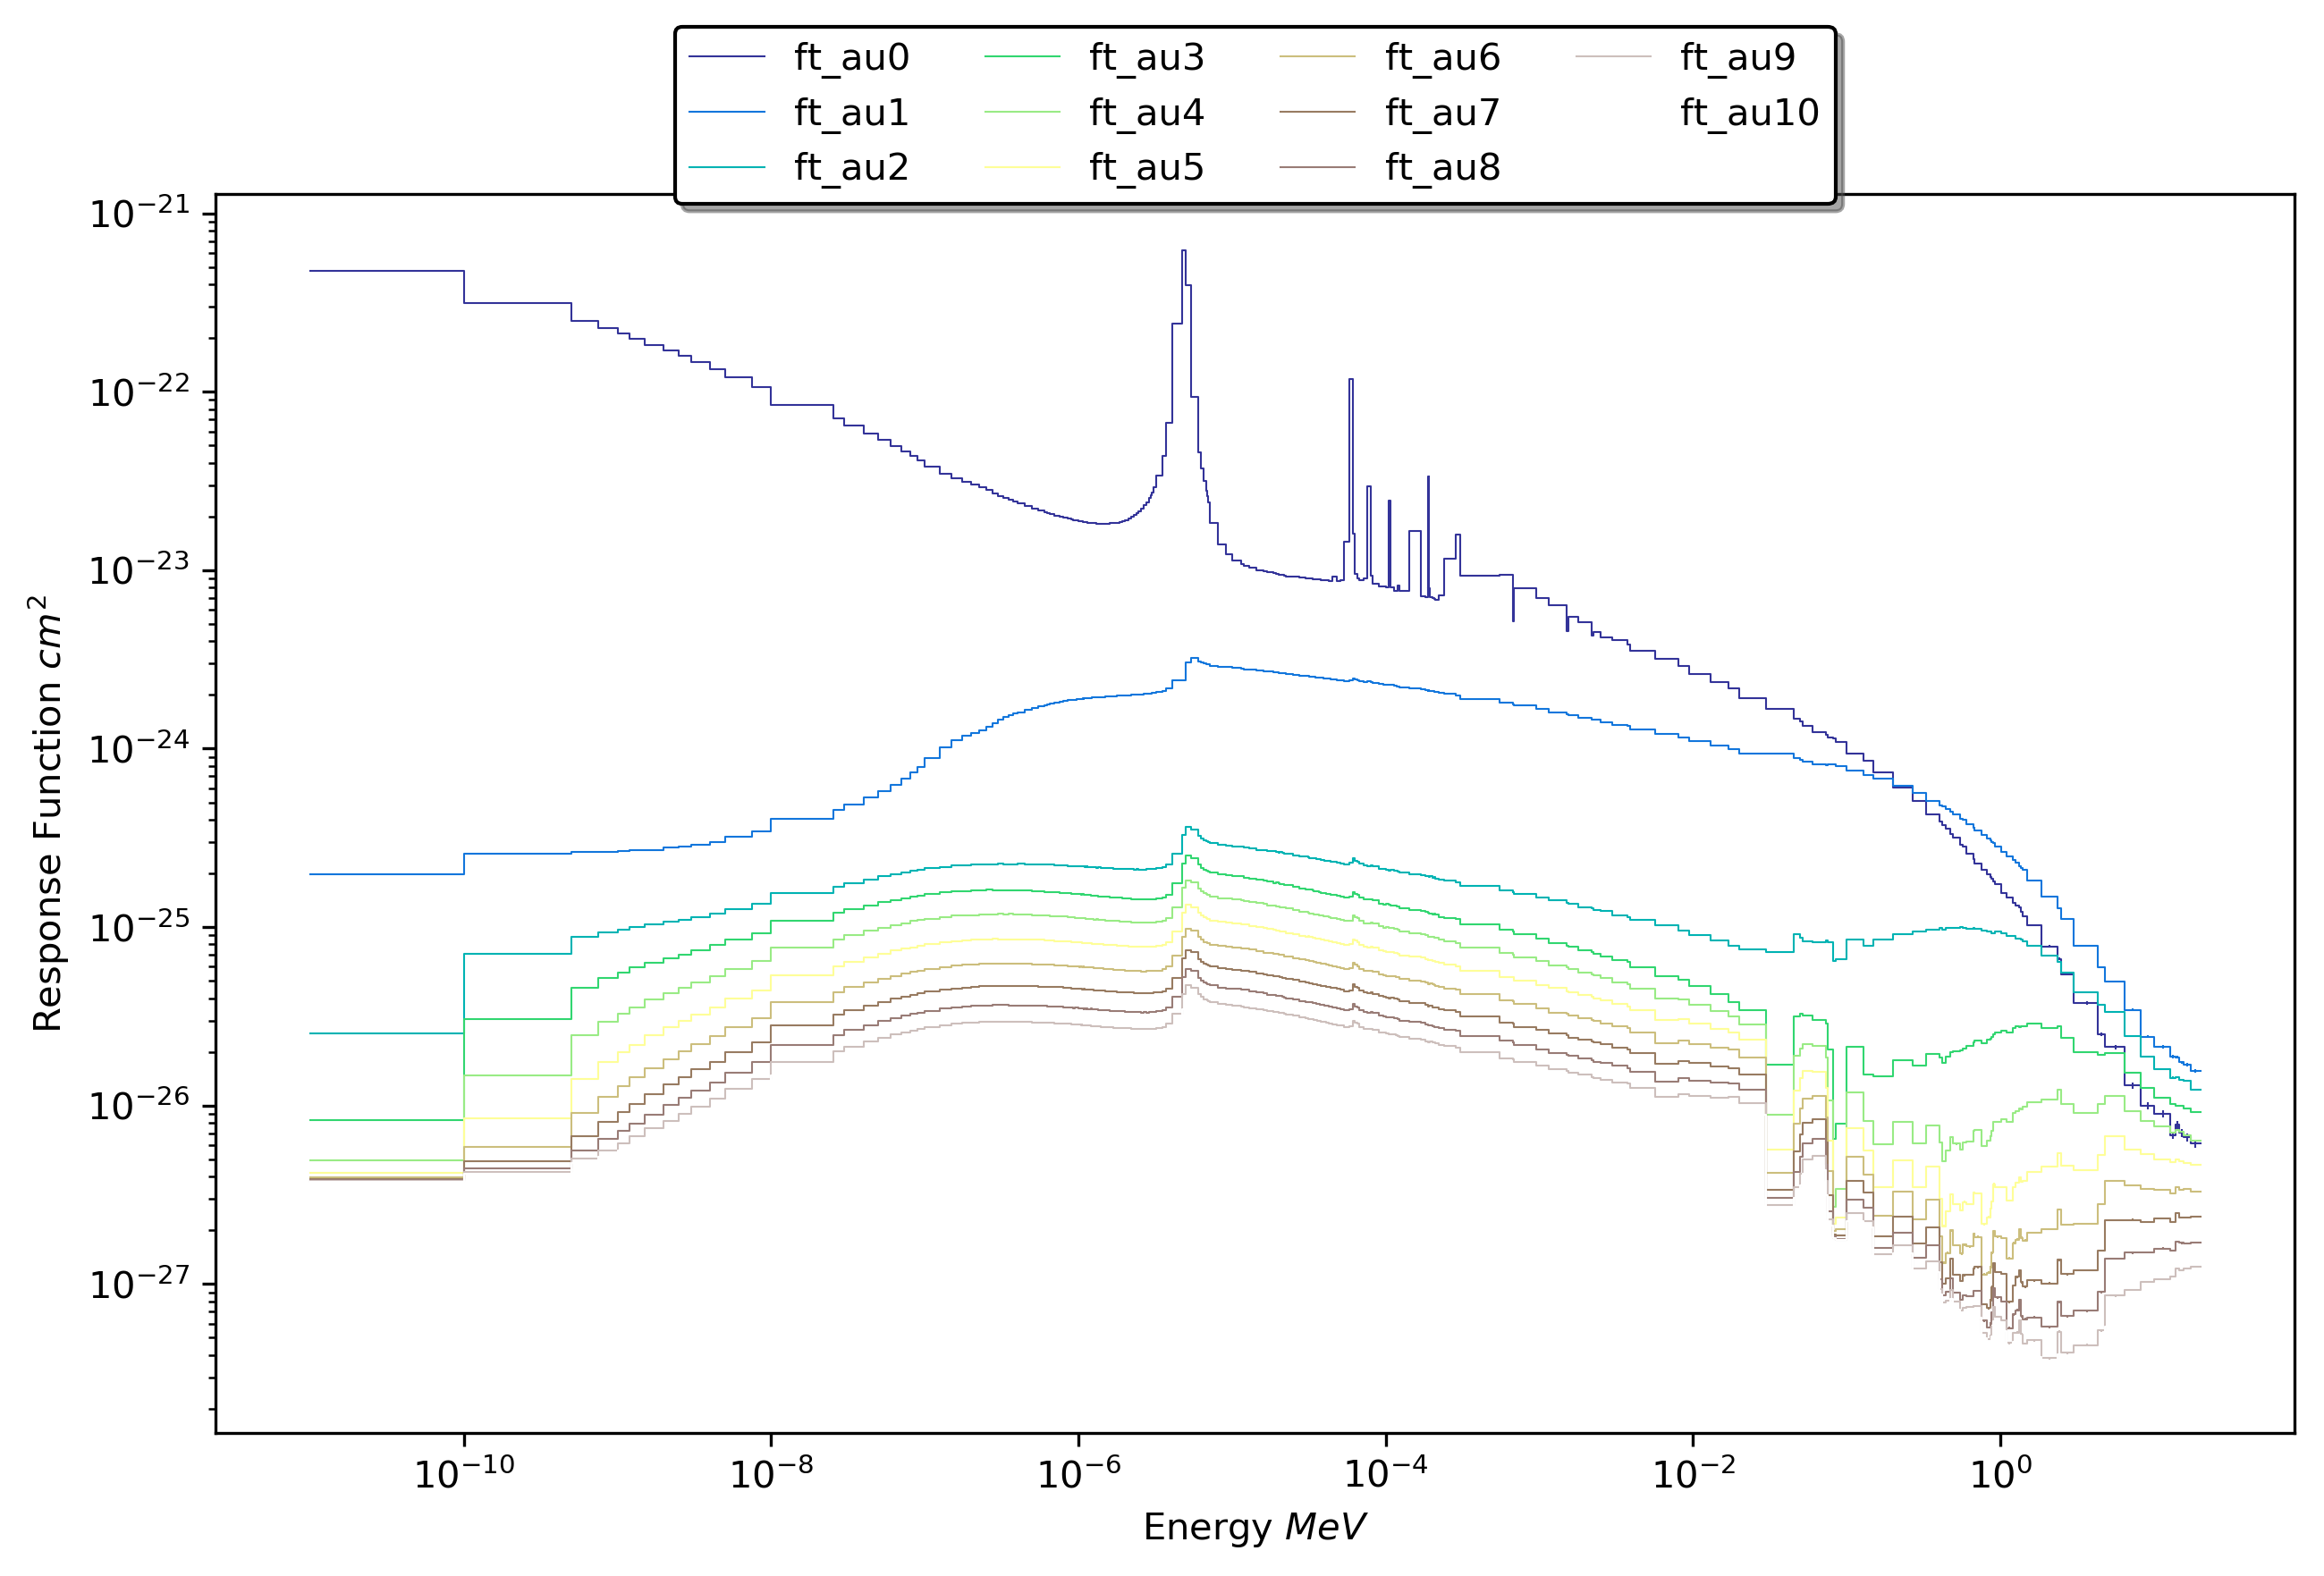
\includegraphics[width = 0.8\textwidth]{ft_au}
\caption{}
\end{figure}

\end{frame}

%%%%%%%%%%%%%%%%%%%%% bonner sphere response functions
\begin{frame}
\frametitle{Bonner Sphere Response Functions}

\begin{figure}
\centering
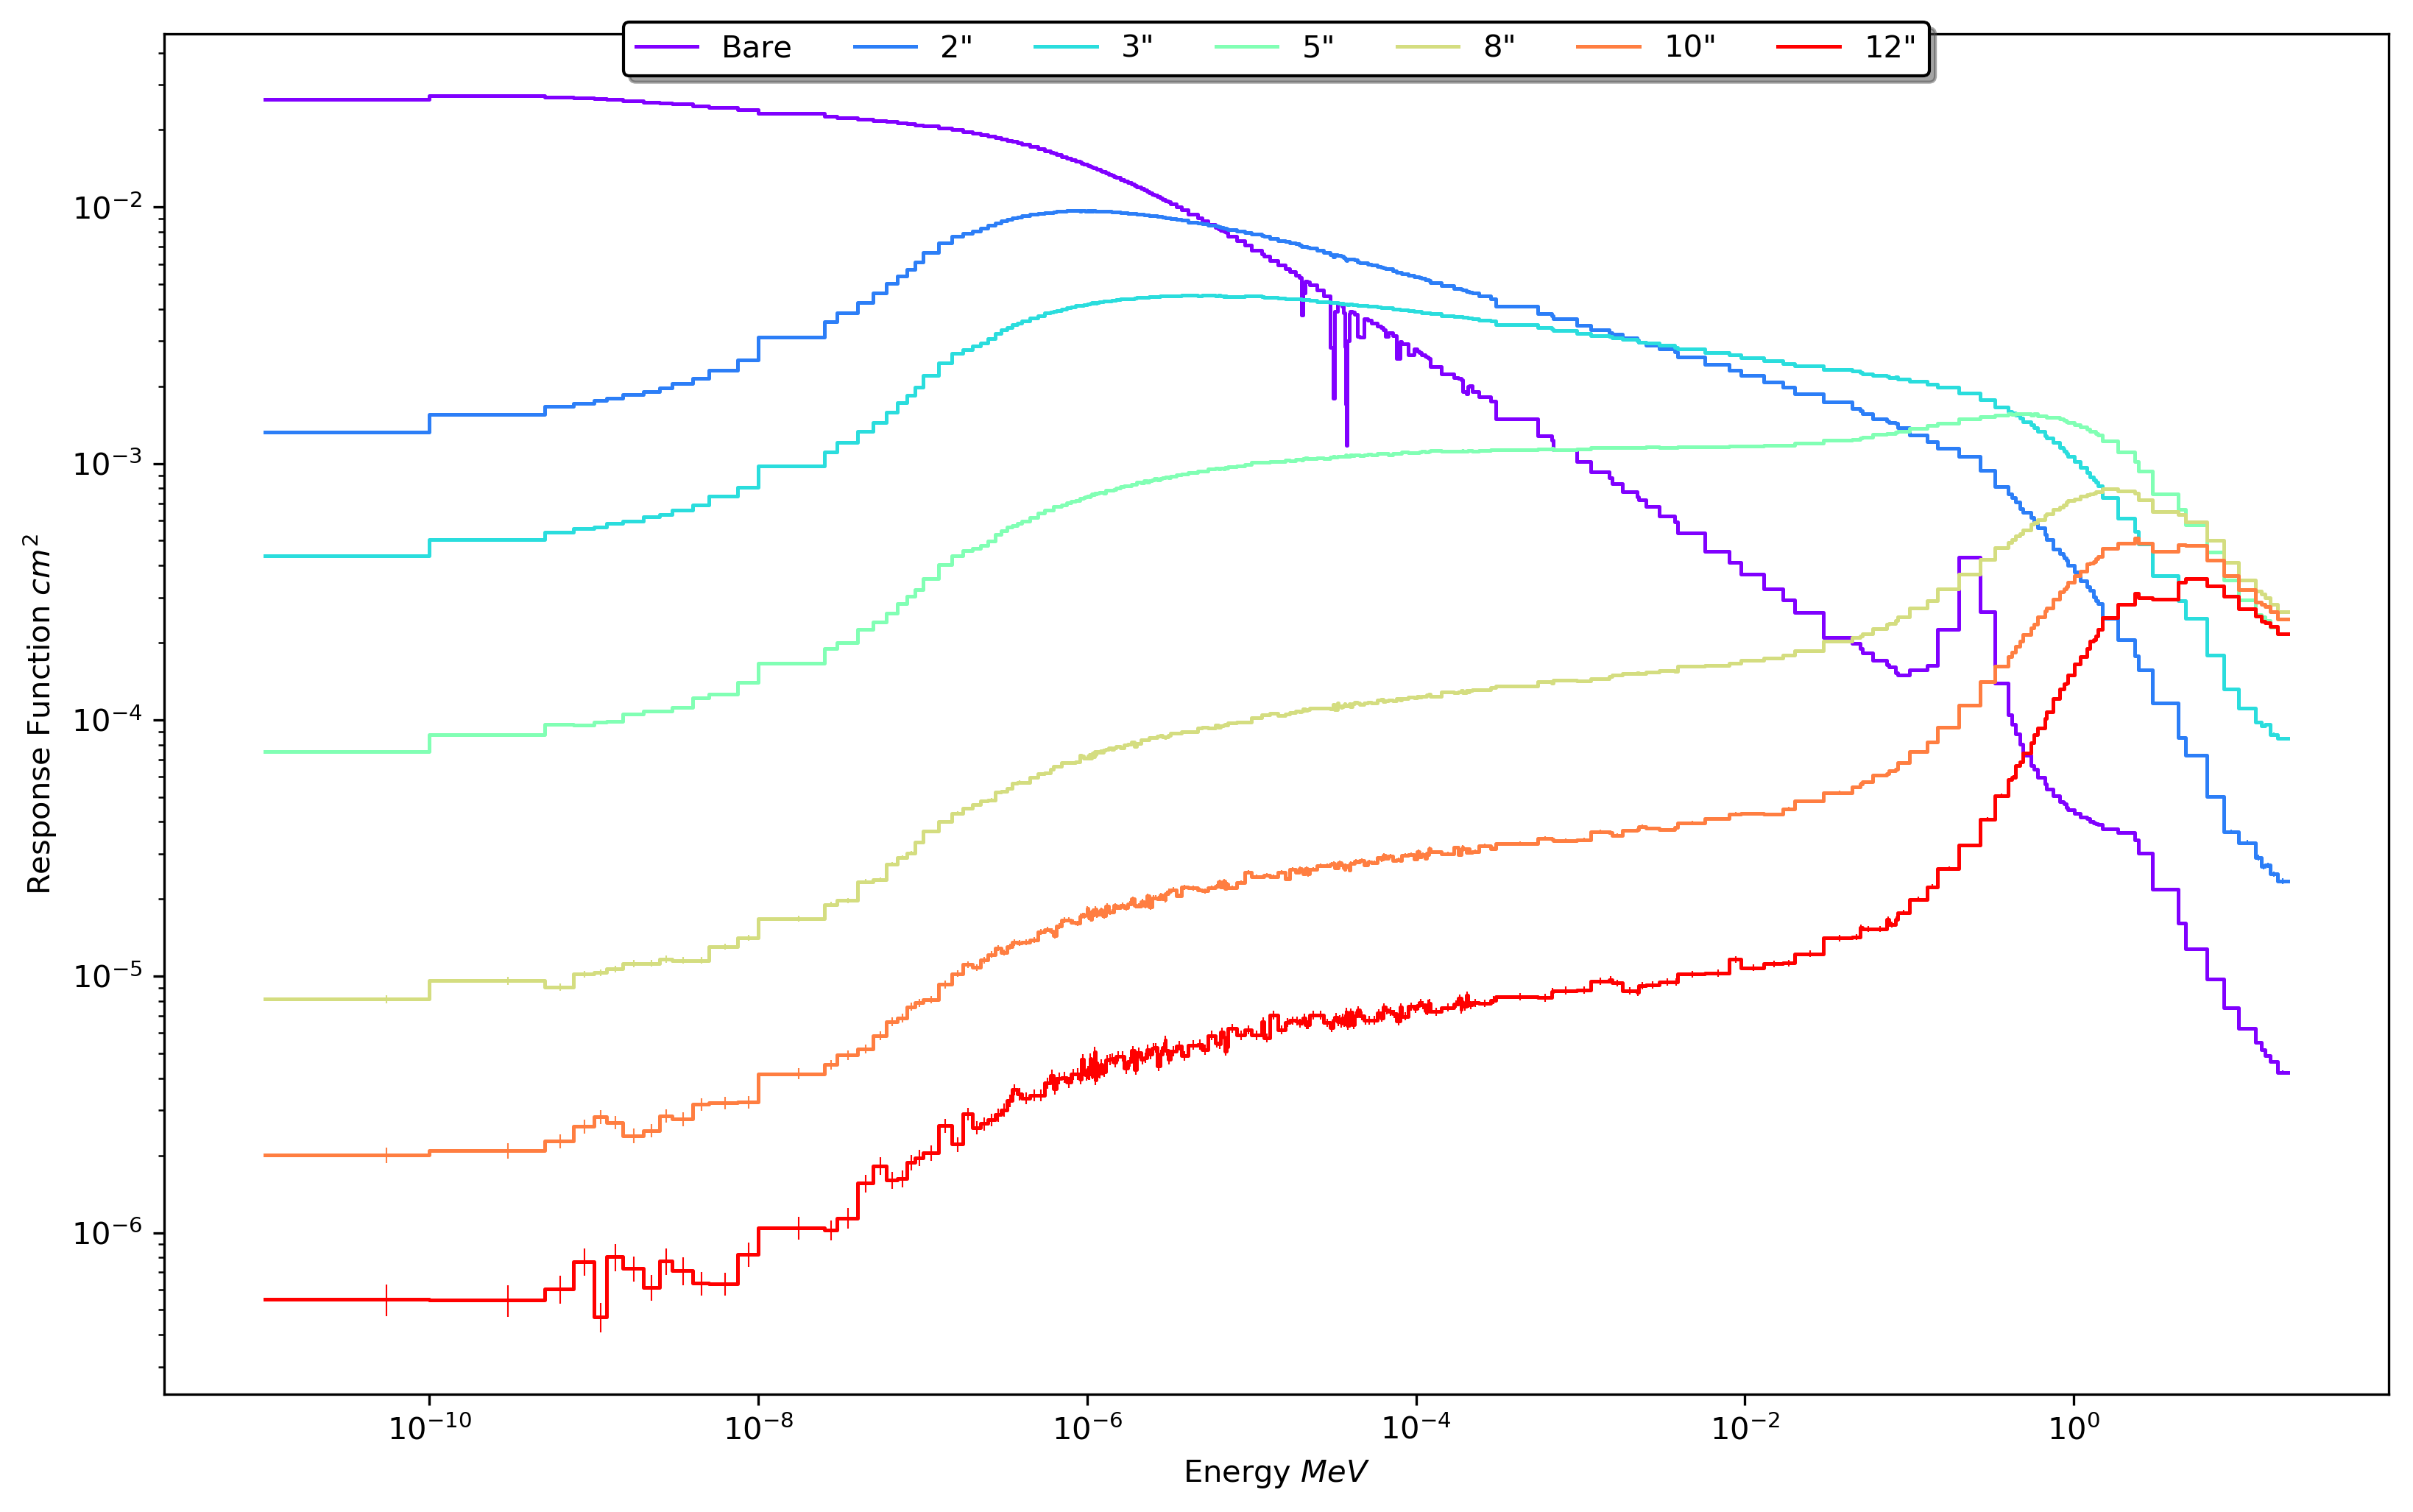
\includegraphics[width = 0.8\textwidth]{bs}
\caption{}
\end{figure}

\end{frame}

%%%%%%%%%%%%%%%%%%%%% experimental procedures: ft
\begin{frame}
\frametitle{Foil Tube Experimental Procedures}

Ran the experiment.

\end{frame}

%%%%%%%%%%%%%%%%%%%%% experimental procedures: bss
\begin{frame}
\frametitle{Bonner Sphere Spectrometer Experimental Procedures}

Ran the experiment.

\end{frame}

%%%%%%%%%%%%%%%%%%%%% gold foil post processing
\begin{frame}
\frametitle{Foil Tube Postprocessing}

\begin{equation}
\label{eqn:a_sat}
A_{sat} = A_{meas} \frac{R_{meas}}{R_{sat} n_a K I_{rel}} ,
\end{equation}

\end{frame}

%%%%%%%%%%%%%%%%%%%%% transient mathematics
\begin{frame}
\frametitle{Capturing Flux Transients}

\begin{equation}
\label{eqn:bateman}
\frac{dN(t)}{dt} = C(t) - \lambda N(t)
\end{equation}

\begin{equation}
\label{eqn:bateman_activity}
\frac{A(t)}{dt} = \lambda (C(t) - A(t)).
\end{equation}

\begin{equation}
\label{eqn:bateman_ratios}
\frac{A(t) / C_{sat}}{dt} = \lambda (\frac{C(t)}{C_{sat}} - \frac{A(t)}{C_{sat}})
\end{equation}

\begin{equation}
\label{eqn:bateman_r_sat}
\frac{R_{sat}(t)}{dt} = \lambda (P_{f}(t) - R_{sat}(t))
\end{equation}

\end{frame}

\begin{frame}
\frametitle{Capturing Flux Transients cont.}

\end{frame}

%%%%%%%%%%%%%%%%%%%%% bss postprocessing
\begin{frame}
\frametitle{Bonner Sphere Postprocessing}

\begin{figure}
\centering
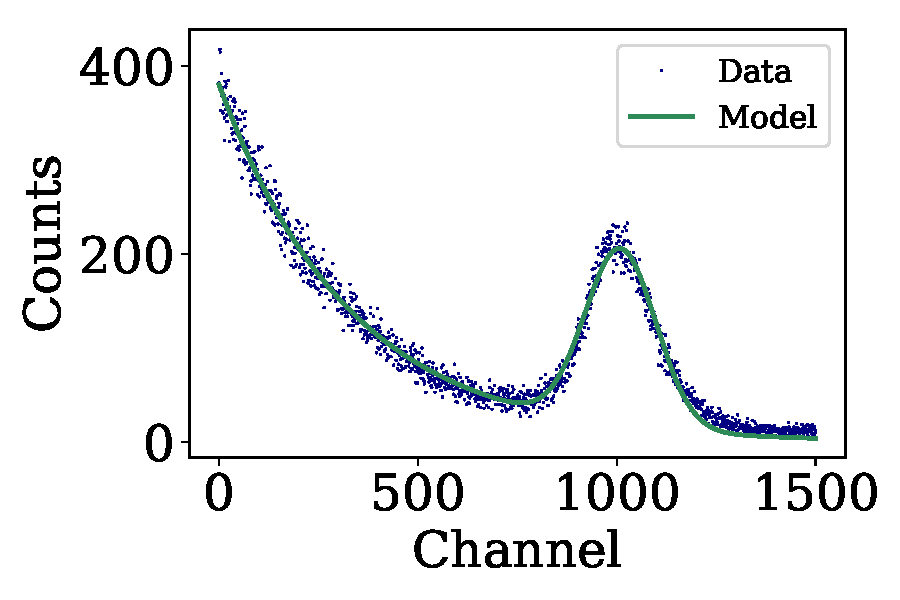
\includegraphics[width = 0.8\textwidth]{bs4_spectrum}
\caption{}
\end{figure}

\end{frame}

%%%%%%%%%%%%%%%%%%%%% response comparison: ft
\begin{frame}
\frametitle{Response Comparison: Foil Tube}

\begin{figure}
\centering
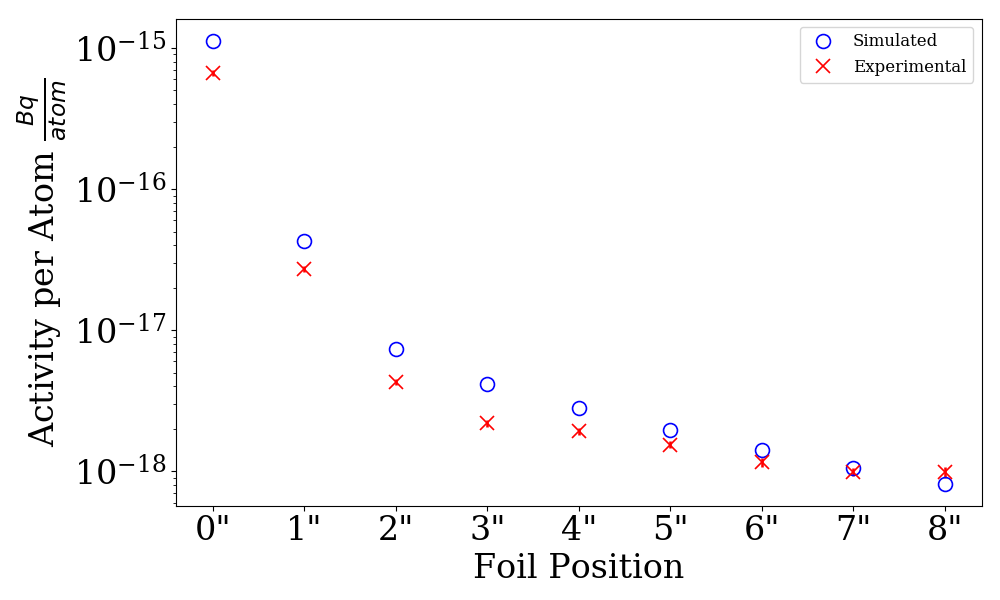
\includegraphics[width = 0.8\textwidth]{compare_activities}
\caption{}
\end{figure}

\end{frame}

%%%%%%%%%%%%%%%%%%%%% response comparison: bss
\begin{frame}
\frametitle{Response Comparison: Bonner Sphere}

\begin{figure}
\centering
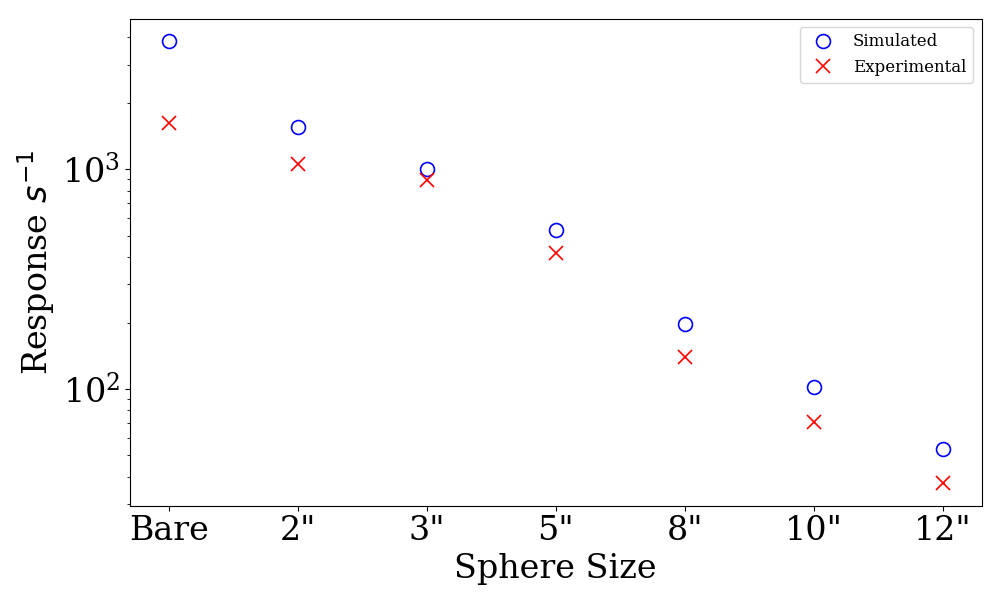
\includegraphics[width = 0.8\textwidth]{compare_countrates}
\caption{}
\end{figure}

\end{frame}

%%%%%%%%%%%%%%%%%%%%% spectral unfolding: parameters
\begin{frame}
\frametitle{Spectral Unfolding Parameters}

Had some parameters.

\end{frame}

%%%%%%%%%%%%%%%%%%%%% spectral unfolding: doroshenko
\begin{frame}
\frametitle{Spectral Unfolding: Doroshenko Directed Divergence}

\begin{figure}
\centering
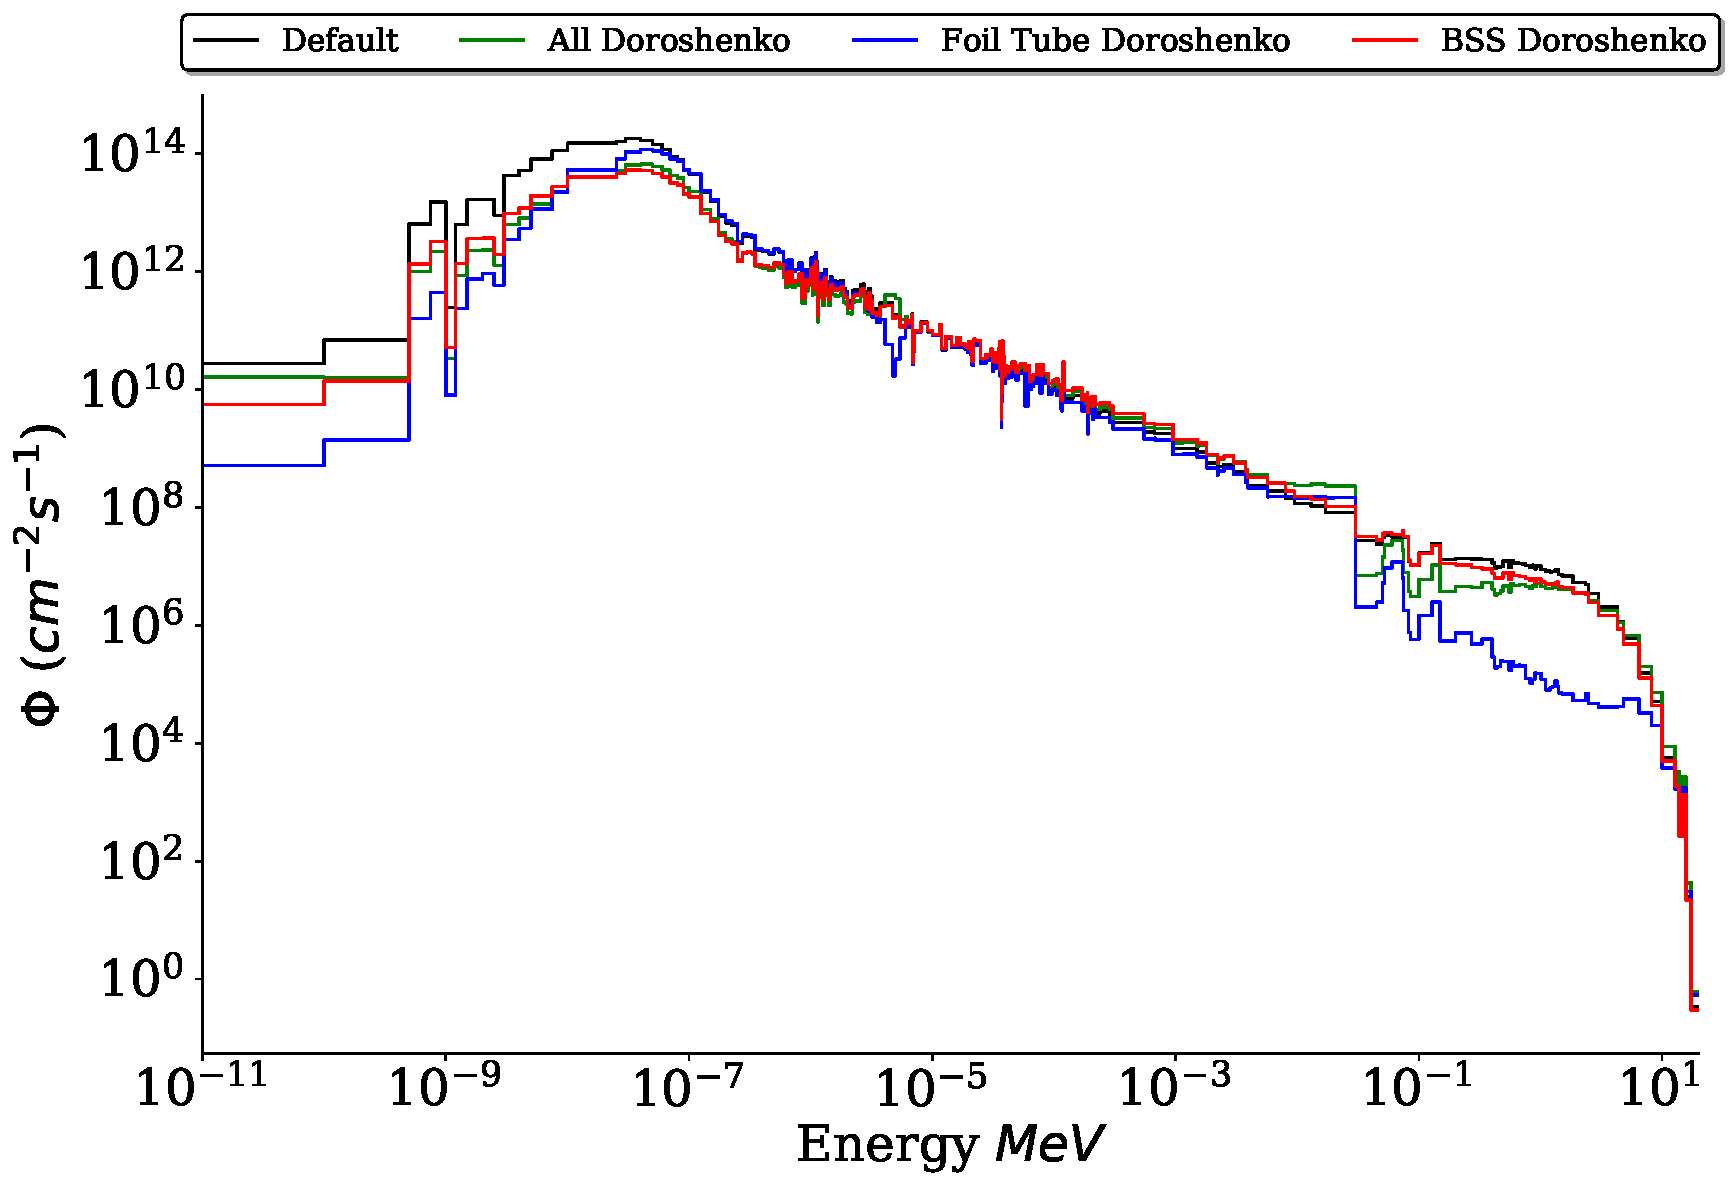
\includegraphics[width = 0.8\textwidth]{unfolded_do}
\caption{}
\end{figure}

\end{frame}

%%%%%%%%%%%%%%%%%%%%% spectral unfolding: gravel
\begin{frame}
\frametitle{Spectral Unfolding: Gravel}

\begin{figure}
\centering
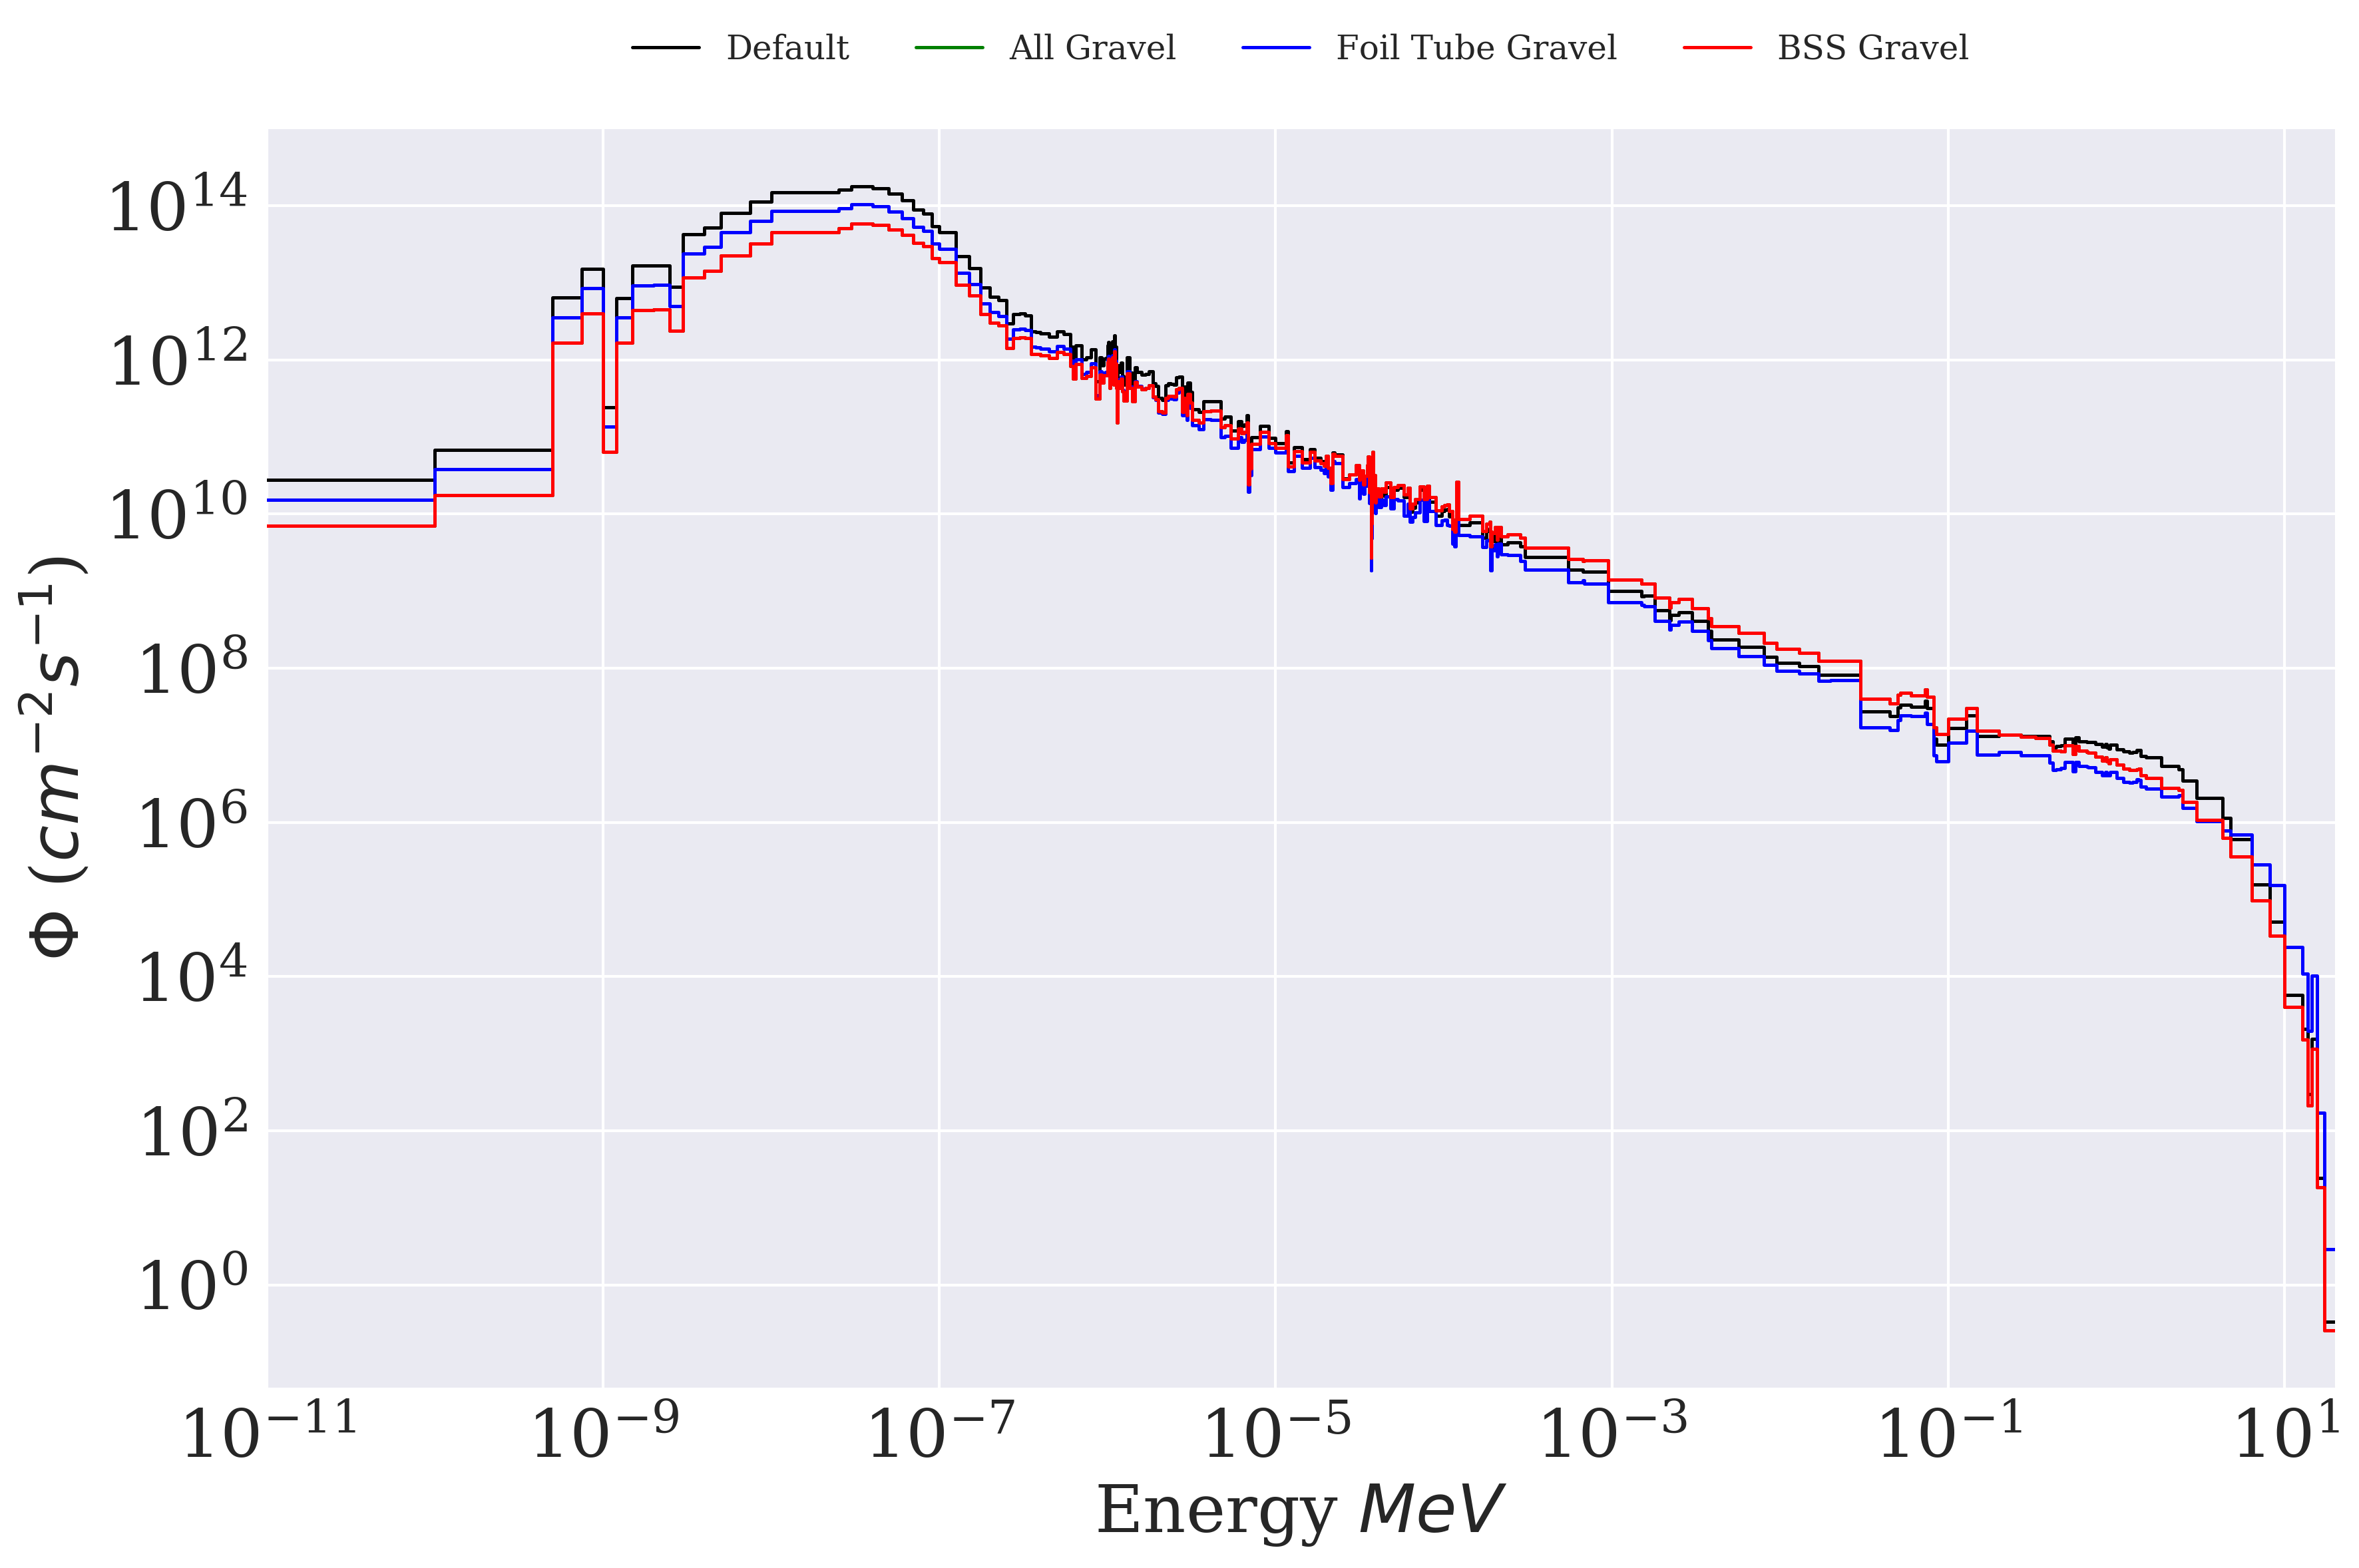
\includegraphics[width = 0.8\textwidth]{unfolded_gr}
\caption{}
\end{figure}

\end{frame}

%%%%%%%%%%%%%%%%%%%%% spectral unfolding: maxed
\begin{frame}
\frametitle{Spectral Unfolding MAXED}

\begin{figure}
\centering
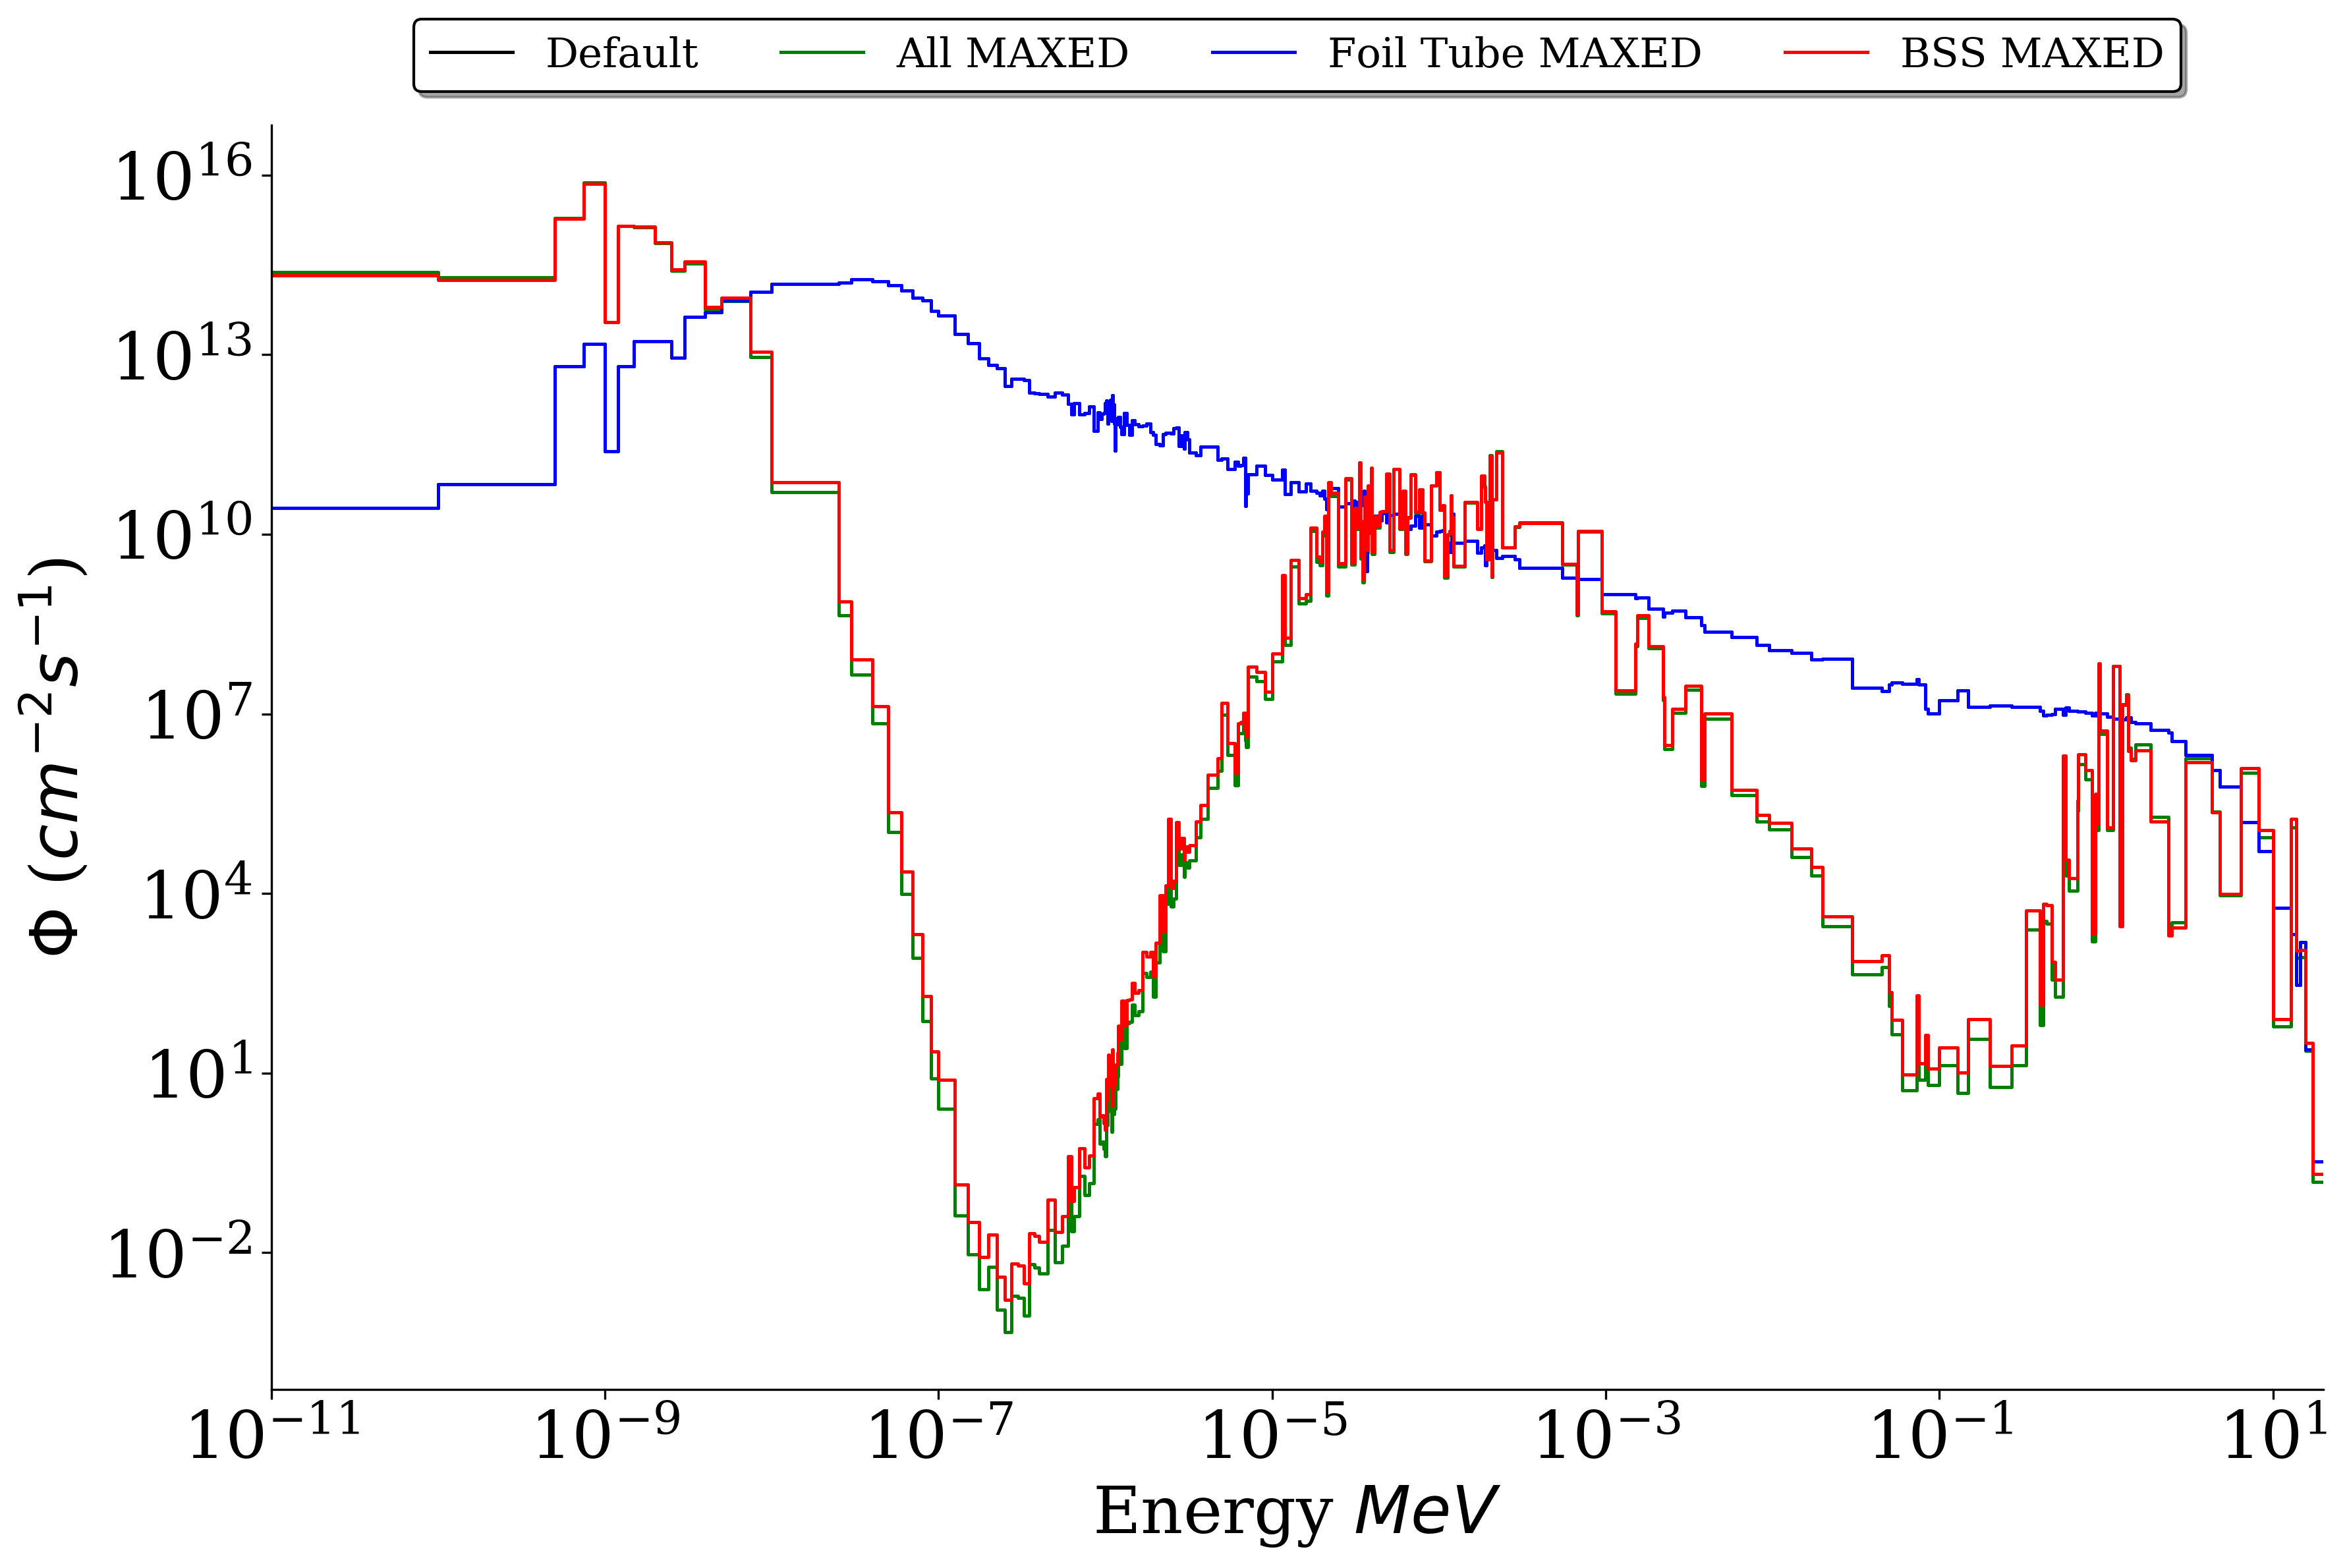
\includegraphics[width = 0.8\textwidth]{unfolded_mx}
\caption{}
\end{figure}

\end{frame}

\begin{frame}
\frametitle{Spectral Unfolding MAXED (Scaled)}

\begin{figure}
\centering
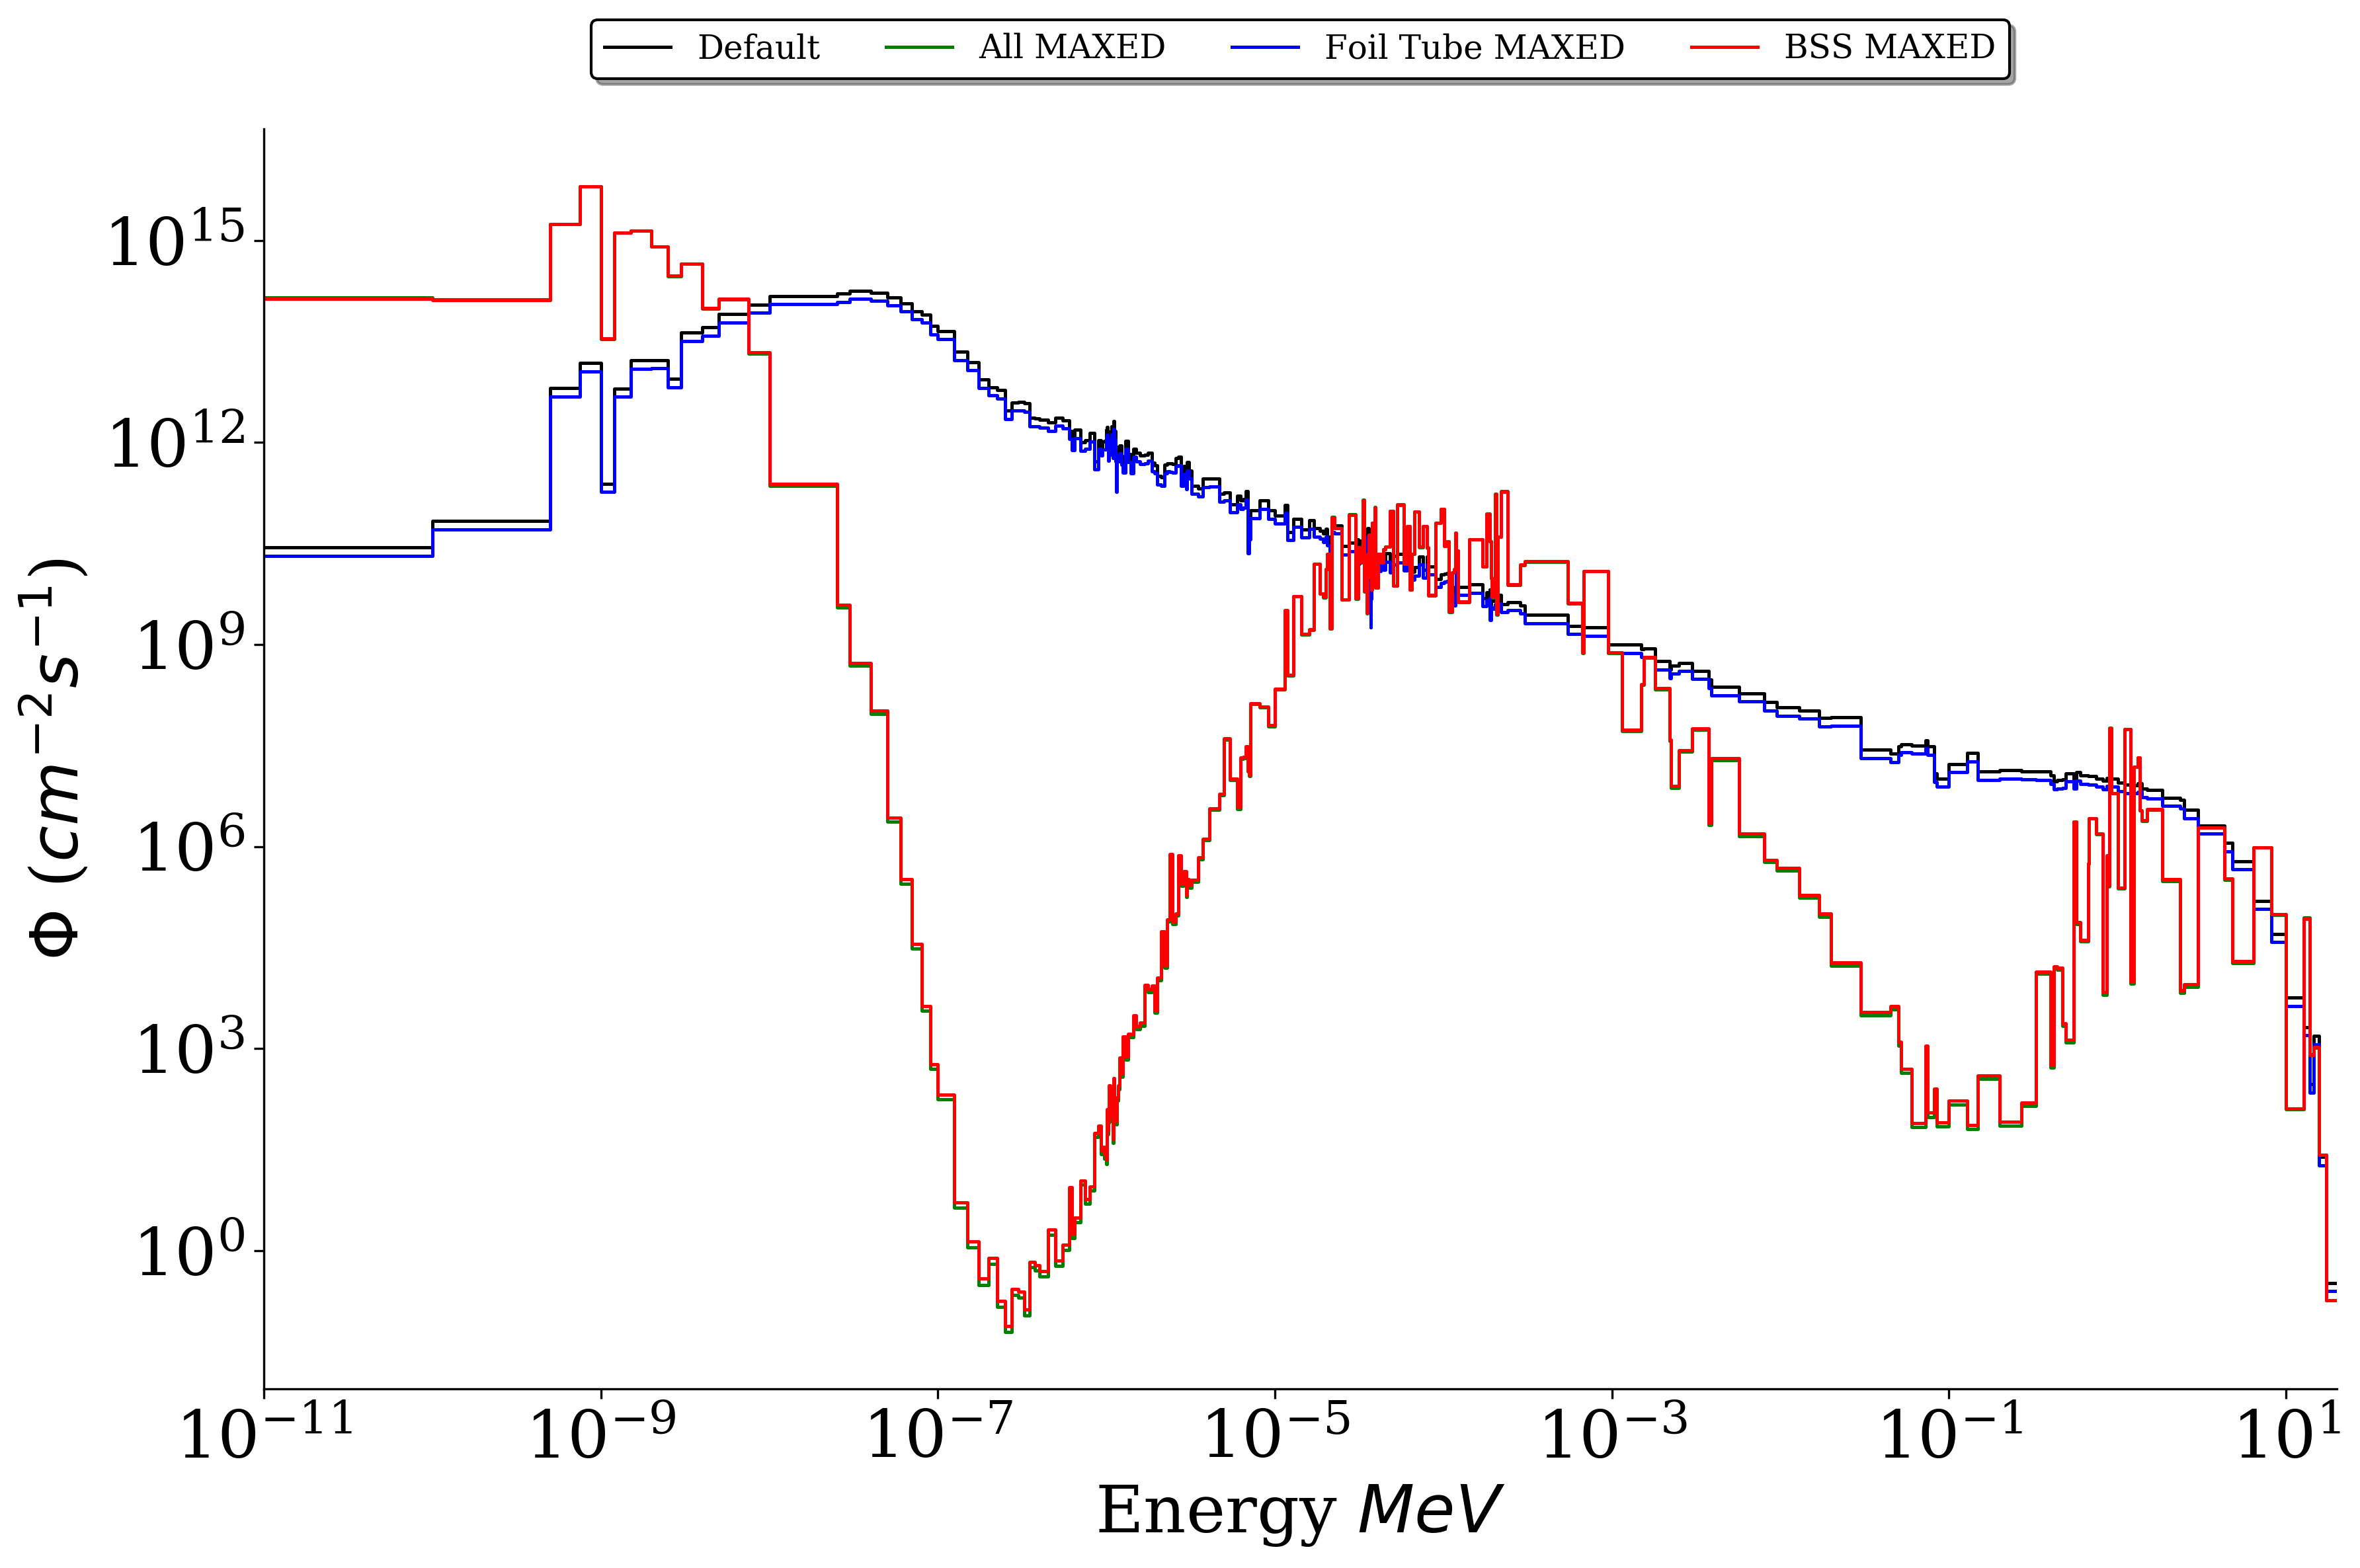
\includegraphics[width = 0.8\textwidth]{unfolded_mx_sc}
\caption{}
\end{figure}

\end{frame}

%%% Conclusions & Future Work (3) ---------------------------------------------------------------------------------------
\section{Conclusions and Future Work}
%%%%%%%%%%%%%%%%%%%%% conclusions
\begin{frame}
\frametitle{Conclusions}

\end{frame}

%%%%%%%%%%%%%%%%%%%%% future work
\begin{frame}
\frametitle{Future Work}

\end{frame}

%%%%%%%%%%%%%%%%%%%%% references
\begin{frame}[t,allowframebreaks]\label{lastframe}
\frametitle{References}
\bibliographystyle{ans}
% make a bibliography.bib file with your references in it
{\scriptsize
\bibliography{bibliography}}
\end{frame}




\end{document}



